%% 
%% ACS project dissertation template. 
%% 
%% Currently designed for printing two-sided, but if you prefer to 
%% print single-sided just remove ",twoside,openright" from the 
%% \documentclass[] line below. 
%%
%%
%%   SMH, May 2010. 


\documentclass[a4paper,12pt,twoside,openright]{report}
%TC:group tabular 1 1

%%
%% EDIT THE BELOW TO CUSTOMIZE
%%

\def\authorname{David Yenicelik\xspace}
\def\authorcollege{ETH Zurich\xspace}
\def\authoremail{yeavid@student.ethz.ch}
\def\dissertationtitle{Parameter Optimization using High-Dimensional Bayesian Optimization}
\def\wordcount{11,513}


\usepackage{epsfig,graphicx,parskip,setspace,tabularx,xspace,verbatim,amssymb,algorithm,url,graphicx,caption,subcaption,amsmath,listings,color,enumitem,afterpage,amsfonts,cleveref,array,multirow,rotating} 

%% DECLARE COMMANDS HERE
\newcommand{\refs}[1]{}
\newcommand{\tb}{\vspace{10pt} \textbf}
\newcommand{\ti}{\textit}
\newcommand{\tx}{\texttt}
\newcommand{\nl}{\\ \\}
\newcommand{\specialcell}[2][c]{%
\begin{tabular}[#1]{@{}c@{}}#2\end{tabular}}
\DeclareFixedFont{\ttb}{T1}{txtt}{bx}{n}{10} % for bold
\DeclareFixedFont{\ttm}{T1}{txtt}{m}{n}{10}  % for normal
\definecolor{deepblue}{rgb}{0,0,0.5}
\definecolor{deepred}{rgb}{0.6,0,0}
\definecolor{deepgreen}{rgb}{0,0.5,0}
\lstset{
language=Python,
basicstyle=\singlespacing\ttm,
captionpos=b,
otherkeywords={self},             % Add keywords here
keywordstyle=\ttb\color{deepblue},
emph={MyClass,__init__},          % Custom highlighting
emphstyle=\ttb\color{deepred},    % Custom highlighting style
stringstyle=\color{deepgreen},
frame=tb,                         % Any extra options here
tabsize=1,                       % sets default tabsize to 2 spaces
stepnumber=1,                       % sets default tabsize to 2 spaces
showstringspaces=false            % 
}
\DeclareMathOperator{\sech}{sech}
\DeclareMathOperator{\csch}{csch}
\DeclareMathOperator{\arcsec}{arcsec}
\DeclareMathOperator{\arccot}{arcCot}
\DeclareMathOperator{\arccsc}{arcCsc}
\DeclareMathOperator{\arccosh}{arcCosh}
\DeclareMathOperator{\arcsinh}{arcsinh}
\DeclareMathOperator{\arctanh}{arctanh}
\DeclareMathOperator{\arcsech}{arcsech}
\DeclareMathOperator{\arccsch}{arcCsch}
\DeclareMathOperator{\arccoth}{arcCoth} 



%% MISC
\setcounter{secnumdepth}{5}
\setcounter{tocdepth}{5}

%% START OF DOCUMENT
\begin{document}


%% FRONTMATTER (TITLE PAGE, DECLARATION, ABSTRACT, ETC) 
\pagestyle{empty}
\singlespacing
% title page information
\begin{titlepage} 

\begin{center}
\noindent
\huge
\dissertationtitle \\
\vspace*{\stretch{1}}
\end{center}

\begin{center}
\noindent
\huge
\authorname \\
\Large
\authorcollege      \\[24pt]

\includegraphics{CUni3.eps}
\end{center}

\vspace{24pt} 

\begin{center}
\noindent
\large
{\it A dissertation submitted to the University of Cambridge \\ 
in partial fulfilment of the requirements for the degree of \\ 
Master of Philosophy in Advanced Computer Science} 
\vspace*{\stretch{1}}
\end{center}

\begin{center}
\noindent
University of Cambridge \\
Computer Laboratory     \\
William Gates Building  \\
15 JJ Thomson Avenue    \\
Cambridge CB3 0FD       \\
{\sc United Kingdom}    \\
\end{center}

\begin{center}
\noindent
Email: \authoremail \\
\end{center}

\begin{center}
\noindent
\today
\end{center}

\end{titlepage} 

\newpage
\vspace*{\fill}

\onehalfspacing
% ******************************* Thesis Declaration ***************************

\begin{declaration}

I hereby declare that except where specific reference is made to the work of 
others, the contents of this dissertation are original and have not been 
submitted in whole or in part for consideration for any other degree or 
qualification in this, or any other university. This dissertation is my own 
work and contains nothing which is the outcome of work done in collaboration 
with others, except as specified in the text and Acknowledgements. This 
dissertation contains fewer than 65,000 words including appendices, 
bibliography, footnotes, tables and equations and has fewer than 150 figures.

% Author and date will be inserted automatically from thesis.tex \author \degreedate

\end{declaration}
\singlespacing
% ************************** Thesis Abstract *****************************
% Use `abstract' as an option in the document class to print only the titlepage and the abstract.
\begin{abstract}

In this thesis, I explore the possibilities of conducting bayesian optimization techniques in high dimensional domains.
Although high dimensional domains can be defined to be between hundreds and thousands of dimensions, we will primarily focus on problem settings that occur between two and 20 dimensions.
As such, we focus on solutions to practical problems, such as tuning the parameters for an electron accelerator, or for even simpler tasks that can be run and optimizated just in time with a common laptop at hand. \\

I follow a systematic methodology, where we identify problems currently occurring with Bayesian Optimization methods.
For this, I take on the following steps: \\

I first provide a theoretic background to the mathematical foundations of Gaussian Processes at hand.
I present the derivation of the surrogate functions as a foundation to better understand what parts of the process can be optimized.
I then shortly discuss the different acquisition functions that are most often used in practice.\\

I continue by exploring different techniques that are currently considered as state-of-the-art. 
Most of these techniques concentrate on doing one of three things.
The most common approach is to do a linear dimensionality reduction.
The second most common approach is to identify variables that rely on each other, and create different Gaussian Processes for each group of variables that depend on each other. \\

I identify the shortcomings of the current methods and present quantitative ways on how we can measure improvements for the goal at hand.
Together with my supervisors, we present a novel algorithm called "BORING" to do Bayesian Optimization at hand.
This algorithm combines the advantages of linear projection methods, but also allows to take into consideration some small perturbations in the target function.
Taking into account smaller perturbations is something that linear reduction models have not taken into account so far.
BORING proves to have all the advantages that other state-of-the-art linear dimensionality reduction algorithms have.
However, BORING improves this state by allowing small perturbations to be taken into account when creating the surrogate function. 
This feature ultimately allows BORING to be more accurate when modelling functions that we want to optimize over. \\

Finally, we evaluate BORING and compare it to the competitive state-of-the-art in Bayesian Optimization.
We do a quantitative analysis by applying the Gaussian Process algorithms on different, well defined functions and measuring the regret during optimization that it achieves.
We do a qualitative analysis by visualizing the predicted surrogate function, and comparing this to the real function.
In addition to that, we do a short experiment on whether the subspace identification method can be used to do feature selection, by choosing the projection in such a way, that the most important features will receive the highest matrix weights. \\

Our main contribution is BORING, an algorithm which is competitive with other state-of-the-art methods in Bayesian Optimization.
The main features of BORING are 1.) the possibility to identify the subspace (unlike most other optimization algorithms), and 2.) to provide a much lower penalty to identify the subspace, as optimization is still the main goal.

\end{abstract}


\pagenumbering{roman}
\setcounter{page}{0}
\pagestyle{plain}

\singlespacing
\tableofcontents
\listoffigures
\listoftables

%\onehalfspacing
\setstretch{1.4}

%% INTRODUCTION
% ************************** Thesis Abstract *****************************
% Use `abstract' as an option in the document class to print only the titlepage and the abstract.
\chapter{Project Proposal for Bachelor Thesis}
\subsection{Motivation}

Tuning hyperparameters is considered a computationally intensive and tedious task, be it for neural networks, or complex physical instruments such as free electron lasers.
Users for such applications could benefit from a 'one-click-search' feature, which would find optimal parameters in as few function evaluations as possible.
This project aims to find such an algorithm which is both efficient and holds certain convergence guarantees.
We focus our efforts on Bayesian Optimization (BO) and revise techniques for high-dimensional BO. \\

\subsection{Background}

In Bayesian Optimization, we want to use a Gaussian Process to find an optimal parameter setting $\mathbf{x^*}$ that maximizes a given utility function $f$.
We assume the response surface to be Lipschitz-continuous. \\

Assume we have observations $ \mathcal{Y} = \{ y^{(1)}, \ldots, y^{(N)} \}$, each evaluated at a point $ \mathcal{X} = \{  \mathbf{x}^{(1)}, \ldots, \mathbf{x}^{(N)} \}$.
The relationship between the observations $y$ and individual parameter settings $\mathbf{x}$ is $y = f \left( \mathbf{x} \right) + \epsilon$ where $\epsilon \sim  \mathcal{N} \left( 0, \sigma^2_n \right)$. Any quantity to be predicted has a subscript-star (e.g. $y_*$ is the function evaluation we want to predict).\\

In it's simplest form, a Gaussian Process is described by the following equation:

\begin{equation}
\begin{pmatrix} y \\
y_* \end{pmatrix} \sim N\Biggl(\mu,\begin{pmatrix} K & K^T_*\\
 K_* & K_{**} \end{pmatrix}\Biggr),
\end{equation}

Where $\mu$ is a mean function, $K = \text{kernel}(\mathbf{X}, \mathbf{X})$, $K_* = \text{kernel}(\mathbf{x_*}, \mathbf{X})$ and $K_{**} = \text{kernel}(\mathbf{x_*}, \mathbf{x_*})$.
We predict any new point $y_*$, (given all previously sampled points $y$) by estimating the probability $ p(y_*|y) \sim N(K_*K^{-1}y,K_{**}-K_*K^{-1}K'_*) $

This, in turn, can be used to build an acquisition function. 
This acquisition function describes where to best sample points next.
Some popular acquisition functions include GP-UCB, Most probable improvement (MPI) and Expected Improvement (EI).
The choice of the acquisition function has great influence on the performance of the optimization procedure.\\

We will talk about the problems and possible solutions for the task at hand in the next section.

\subsection{Scope of the Project}

Bayesian optimization suffers from the curse of dimensionality. 
The goal of this project is to arrive at a solution that resolves the curse of dimensionality for the specific task with regards to Bayesian optimization.
This project includes, but is not limited to the following methods.\\

\begin{enumerate}
\item \cite{Tripathy}
Assume $f(x) \approx g( \mathbf{W}^T x)$ where $ \mathbf{W} \in \mathbb{R}^{D \times d} $ and $D >> d$.
We assume that $ \mathbf{W} $ is orthogonal.

This algorithm does not require gradient-information (thus, easier to implement, and robust to noise).
The standard-deviation, kernel parameters and  $ \mathbf{W} $ can be found iteratively.
First we fix $ \mathbf{W} $, and optimize over the standard-deviation, kernel parameters.
Then we fix the standard-deviation, kernel parameters. and optimize over $ \mathbf{W} $.
We repeat this procedure until the change of the log-likelihood between iterations is below some $ \epsilon_l $.

\item \cite{Rolland}
Assume $f(x) = f^{(1)}( x^{(1)} )  + f^{(2)}( x^{(2)} ) + \ldots + f^{(M)}( x^{(M)} )$ where $ x^{(i)} \in \mathcal{X}^{(i)} \subseteq \mathcal{X}$, i.e. each function component  $f^{(i)}$ takes some lower-dimensional subspace as the input.
The lower-dimensional subspaces may overlap.
The mean and covariance of $f(x)$ is then the sum of the individual component's means and covariances.

An additive decomposition (as described above) can be represented by a dependency graph. The dependency graph is built by joining variables $i$ and $j$ with an edge whenever they appear together within some set $x(k)$. 

The goal is to maximize an acquisition function $ \phi_t(x) = \sum_{i=1}^M \phi_t^{(i)} ( x^{(i)} )$. 
This maximization is achieved by maximizing the probability of Markov Random Fields within the graph.
A junction tree is created from the graph, which is then used to find the global maximum of the acquisition function.

The dependencies between the variable-subsets are represented through a graph, which can be learned through Gibbs sampling.
This, in turn, is used to create a kernel for the GP.

% TODO: cite rembo!
\item \cite{Wang}
A function $f : \mathbf{R}^D \rightarrow \mathbf{R}$ is said to have effective dimensionality $d_e$ (where $d_e < D$), if there exists a linear subspace $\mathcal{T}$ of dimension $d_e$ such that for all $ x_\top \in \mathcal{T} \subset \mathbf{R}^D $ and $x_\perp \in \mathcal{T_\perp} \subset \mathbf{R}^D $, we have $ f(x) = f(x_\top +x_\perp ) = f(x_\top)$.
$\mathcal{T^\perp}$ is the orthogonal complement of $\mathcal{T}$.

Assume $ f : \mathbf{R}^D \rightarrow \mathbf{R} $ has effective dimensionality $d_e$.
Given a random matrix $ \mathbf{A} \in \mathbf{R}^{D \times d} $ (where $d \geq d_e$) with independent entries sampled fom $ \mathcal{N}(0, 1) $.
For any $ x \in \mathbf{R}^D $, there exists a $y \in \mathbf{R}^d $ such that $ f(x) = f(\mathbf{A} y ) $.
We now only need to optimize over all possible $y \in \mathbf{R}^d$, instead of all possible $x \in \mathbf{R}^D $.


\begin{figure}[h]
\centering
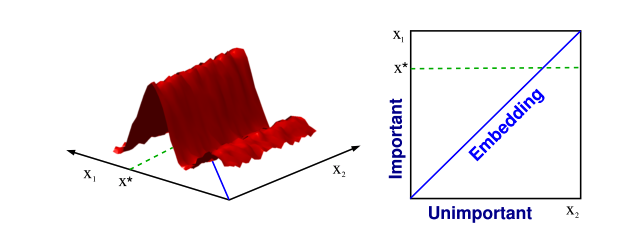
\includegraphics[width=0.5\textwidth]{./figs/src/Embedding_optimization.png}
\caption{ This function in D=2 dimesions only has d=1 effective dimension. Hence, the 1-dimensional embedding includes the 2-dimensional function’s optimizer. It is more efficient to search for the optimum along the 1-dimensional random embedding than in the original 2-dimensional space}
\end{figure}

\end{enumerate}

If, for some reason, finding an active subspace or an effective lower dimension is not possible, we are open to adapt the procedure of optimization.

%********************************** %First Section  **************************************
\chapter{Bayesian Optimization in high dimensions}

Many of today's problems can be boiled down to some flavour of black box optimization. 
Such problems include neural architecture search, hyper-parameter search for neural networks, parameter optimization for electron accelerators, or drone parameter optimization using safety constraints (CITE Johannes). \\

Bayesian optimization methods are a class of sequential black box optimization methods, where we learn a surrogate function surface using a Gaussian prior, and a Gaussian likelihood function.
Combining the prior and the likelihood results in the Gaussian Posterior, which we then can be used as a surface over which we try to optimize. \\

Bayesian optimization is a method that has increasingly gained attention in the last decades, as it requires relatively few points to find an appropriate response surface for the function over which we want to optimize over.
It is a sequential model based optimization function, which means that we choose the best point $x^*_i$ given all previous points $x^*_{i-1}, x^*_{i-2}, \ldots, x^*_{0}$.
Given certain acquisition functions, it offers a good mixture between exploration and exploitation from an empirical standpoint. \\

Bayesian optimization is a method that has increasingly gained success in finding a good mixture between exploration the search space (finding new hyper-parameter configurations that outperform all existing configurations), and exploiting currently found best configurations (using the best learned hyper-parameter configurations to get utility out of the system). \\

However, as machine learning algorithm, and other problems become more complex, bayesian optimization needs to cope with the increasing number of dimensions that define the search space of possible configurations.
Because BO methods loose effectiveness in higher dimensions, this work deals with methods that work in higher dimensions.

\section{Gaussian Processes}
In Bayesian Optimization, we want to use a Gaussian Process to find an optimal parameter setting $\mathbf{x^*}$ that maximizes a given utility function $f$.
We assume the response surface to be Lipschitz-continuous. \\

Assume we have observations $ \mathcal{Y} = \{ y^{(1)}, \ldots, y^{(N)} \}$, each evaluated at a point $ \mathcal{X} = \{  \mathbf{x}^{(1)}, \ldots, \mathbf{x}^{(N)} \}$.
The relationship between the observations $y$ and individual parameter settings $\mathbf{x}$ is $y = f \left( \mathbf{x} \right) + \epsilon$ where $\epsilon \sim  \mathcal{N} \left( 0, \sigma^2_n \right)$. Any quantity to be predicted has a subscript-star (e.g. $y_*$ is the function evaluation we want to predict).\\

In it's simplest form, a Gaussian Process is described by the following equation:

\begin{equation}
\begin{pmatrix} y \\
y_* \end{pmatrix} \sim N\Biggl(\mu,\begin{pmatrix} K & K^T_*\\
 K_* & K_{**} \end{pmatrix}\Biggr),
\end{equation}

Where $\mu$ is a mean function, $K = \text{kernel}(\mathbf{X}, \mathbf{X})$, $K_* = \text{kernel}(\mathbf{x_*}, \mathbf{X})$ and $K_{**} = \text{kernel}(\mathbf{x_*}, \mathbf{x_*})$.
We predict any new point $y_*$, (given all previously sampled points $y$) by estimating the probability $ p(y_*|y) \sim N(K_*K^{-1}y,K_{**}-K_*K^{-1}K'_*) $

This, in turn, can be used to build an acquisition function. 
This acquisition function describes where to best sample points next.
Some popular acquisition functions include GP-UCB, Most probable improvement (MPI) and Expected Improvement (EI).
The choice of the acquisition function has great influence on the performance of the optimization procedure.\\

We will talk about the problems and possible solutions for the task at hand in the next section.

\subsection{Derivation of the Gaussian Process Formula}
The prior for the Gaussian Process it the following (assuming a 0-mean-prior).

\begin{equation}
u \sim GP(0, k(x, x'))
\end{equation}

Because $u$ is a random variable, it's probably distribution is given by a normal distribution (as determined by the Gaussian Process):

\begin{equation}
p(u) = N ( 0, K )
\end{equation}

Now we go over to observing some data $ X = \{ (x_1, y_1), \ldots, (x_n, y_n) \} $ where $y$ has some noise term $\epsilon$ such that $y = u(x) + \epsilon$.
We assume that $\epsilon$ is normally distributed around $0$ with $\sigma$ standard deviation.
This means that the likelihood takes on the following form:

\begin{equation}
p(y | x, u) = N (u, \sigma^2 I)
\end{equation}

% https://stats.stackexchange.com/questions/84058/derivation-of-predictive-distribution-of-gaussian-process

Now we want to derive the posterior of the Gaussian Process, given the likelihood and the prior.
We use Bayes rule to derive this

\begin{align}
p(u | x, y) &= \frac{ p(y | x, u) p(u) }{p(y | x)}
& = N( K(K +\sigma^2 I)^{-1}y, \sigma^2 (K + \sigma^2 I)^{-1} K )
\end{align}

At this point, we want to create a surrogate embeddings, that predicts $y_*$ for any possible given $x_*$. 
We refer to this as the surrogate response surface.

We use the following formula to derive the posterior distribution for a given predictor $y_*$.

\begin{equation}
\begin{pmatrix} y \\
y_* \end{pmatrix} \sim N\Biggl(\mu,\begin{pmatrix} K & K^T_*\\
 K_* & K_{**} \end{pmatrix}\Biggr),
\end{equation}

To numerically calculate this, one uses the Matrix Inversion Lemma (CITE Murphy Chapter 4.3 110-111)


\section{Acquisition Functions}

Given the above formula for the posterior mean $\mu$ and the poster variance $\sigma^2$, Bayesian Optimization uses an acquisition function to optimize over.
We quickly present some of the most common acquisition functions.

% Most formulae taken from "A tutorial on Bayesian optimization of expensive cost functions, with application to active user modeling and hierarchical reinforcement learning

\subsection{Upper Confident Bound (UCB)}
(CITE Krause Srinivas) about how acquisition function is guaranteed to find best config after awhile.

The upper confidence bound allows the user to control exploitation and exploration through a parameter $\beta > 0$, which can be chosen as CITE PAPER, to offer optimality guarantees.

\begin{equation}
UCB(x) = \mu(x) + \beta \sigma(x)
\end{equation}

Here, the functions $\mu$ and $\sigma$ are the predicted mean and variance of the Gaussian Process Posterior.

\subsection{Probability of Improvement (PI)}
The (maximum) probability of improvement always selects the point which has the highest potential to maximise the function. 
The downside to this policy is that this leads to exploitation, which can be controlled by a parameter $\xi > 0$.

\begin{align}
    PI(x) & = P( f(x) \geq f(x^+) + \xi ) \\
    & = \Phi ( \frac{\mu(x) - f(x^+) - \xi}{\sigma(x)}  ) 
\end{align}


\subsection{Expected Improvement (EI)}

"CITE A tutorial on Bayesian optimization of expensive cost functions, with application to active user modeling and hierarchical reinforcement learning"
\begin{align}
    EI(x) =
    \begin{dcases}
        ( \mu (x) - f(x^+) \Phi(Z) \sigma (x) \phi (Z) )  & \text{ if } \sigma (x) > 0 \\
        0 & \text{ if } \sigma (x) = 0
    \end{dcases} \\
\end{align}

\begin{equation}
    Z = \frac{\mu (x) - f(x^+) }{\sigma(x)}
\end{equation}

Given one of the above acquisition functions, we then use an optimizer such as $L-BFGS$, to find an approximate global maximum of the respective function.
The combination of Gaussian Processes and Acquisition function together result in a Bayesian Optimization algorithm, which has a prior assumption about the function to be learned, and uses datasamples to create a likelihood to further refine the posterior of the function assumption.

\section{Resources}
(CITE https://github.com/SheffieldML/GPy)
We will use "GPy: A Gaussian process framework in python" and "CITE https://github.com/SheffieldML/GPyOpt" by the Sheffield Machine Learning Group.
In addition to that, the febo framework developed by Johannes Kirschner from the Learning and Adaptive Systems group at ETH Zurich.
We use pytest to write tests (CITE).

\chapter{Related Work} \label{ch3}

This section covers current methods solving Bayesian Optimization in high dimensions that are considered state-of-the-art.
This is not an exhaustive review. 
For each algorithm, I discuss the effectiveness with regards to the dataset or function that the respective paper does the evaluation on.

Conventions that I use is the following:

\begin{enumerate}
\item $f$ is the real function to be approximated / optimized.
\item $g$ and any subscripted or superscripted derivative of $g$ is a component that one uses to approximate $f$.
\item Anything that has a "hat" on (caret symbol on f is $\hat{f}$ ), refers to an empirical estimate. 
\end{enumerate}

I will focus on three categories of Bayesian Optimization algorithms: Algorithms that make use of a projection matrix, algorithms that, algorithms that exploit additive substructures and "additional approaches" that are uncategorised.

\section{Projection matrix based algorithms}

Generally, for this family of algorithms, the approximation is a function of $f(x) \sim g(Ax)$, where the properties and identification of $A$ are algorithmic specific.

\subsection{Active learning of linear subspace}

\begin{algorithm}
\caption{Simultaneous active learning of functions and their linear embeddings (pseudocode) :: Active learning of linear subspace \citep{Garnett2013}}

\begin{algorithmic} 
\REQUIRE $d, D;$ kernel $\kappa$, mean function $\mu$; prior $p(R)$ 
\STATE $X \leftarrow \emptyset$
\STATE $Y \leftarrow \emptyset$

\WHILE{budget not depleted}
\STATE $ q(R) \leftarrow \text{LAPLACEAPPROX}( p(R | X, Y, \kappa, \mu) ) $
\STATE $ q(f) \leftarrow  APPROXMARGINAL( p(f | R), q(R)) $
\STATE $ x_* \leftarrow OPTIMIZEUTILITY( q(f), q(R) )$
\STATE $ y \leftarrow OBSERVE( f( x_* ) ) $
\STATE $ X \leftarrow [X; x_*] $
\STATE $ Y \leftarrow[Y; y_*] $
\ENDWHILE

\RETURN $q(R), q(f)$
\end{algorithmic}

\end{algorithm}

\citep{Garnett2013} The assumption of this algorithm is that $f$ depends only on $ x := uR^T $ with $ R \in \mathbf{R}^{d \times D}$, $ u \in \mathbf{R}^d $ and where $d << D$. 
The algorithm learns a projection matrix $R$ and the surrogate function$g(u)$, with $f(x) \sim g(u) $. \\

The \textbf{Laplace approximation} for $R$ is using the mode of the probability distribution $\log P (R | D) $ as a mean, and the covariance is taken as the inverse Hessian of the negative logarithm of the posterior evaluated at the mean of the distribution.
Together, this describes the probability distribution $p(R|X, Y, \kappa, \mu )$, where $\mu$ is the mean function, and $\kappa$ is the covariance function.\\

% TODO: be more accurate here
The \textbf{approximate marginal} subroutine is a novel method proposed in the paper that integrates over the different parameters in the paper.
This marginal approximation does a local expansion of $q(x_* | \theta) $ to $p(x_* | D, \theta)$. \\

The \textbf{optimization of utility} (choice of next best point) is done using Bayesian Active Learning by disagreement, where the utility function is the expected reduction in the mutual information, as opposed to uncertainty sampling reducing entropy, which  is not well defined for all values. \\

The metrics used in this paper are negative log-likelihoods for the test points, and the mean symmetric kullback leiber divergence between approximate and true posteriors.
The proposed method always outperforms the naive MAP method for the presented functions close to a factor of 2 for both loss functions.
Tests are conducted on a real, and synthetic dataset with up to $D = 318$ and selecting $N = 100$ observations. 

\subsection{High dimensional Gaussian bandits}

\citep{Djolonga2013} This model assumes that there exists a function $g : \mathbf{R}^k \implies [0, 1]$ and a matrix $A \in \mathbf{R}^{d \times D}$ with orthogonal rows, such that $f(x) \sim g(Ax) $. Assume $g \in \mathcal{C}^2$. 
% Assume that $B = \mathbf{B}^D (1 + \epsilon ) $.
% We want to maximize $f: B \implies [0, 1] $.\\

\begin{algorithm}
\caption{The SI-BO algorithm \citep{Djolonga2013}}

\begin{algorithmic} 
\REQUIRE $m_X, m_{\Phi}, \lambda, \epsilon, k$, oracle for the function $f$, kernel $\kappa$ 

\STATE $C \leftarrow m_X $ samples uniformly from $\mathbb{S}^{d-1}$

\FOR{$ i \leftarrow 1$ to $m_X$}
\STATE $\Phi_i \leftarrow m_{\Phi}$ samples uniformly from $\{ -\frac{1}{\sqrt{m}}, \frac{1}{\sqrt{m}} \}^k$
\ENDFOR

\STATE $ y \leftarrow $ (compute using Equation 1 -- INSERT Eq 1 here, or create a summary of all important equations here)

\STATE select $z_i$ according to a UCB acquisition function, evaluate $f$ on it, and add it to the datasamples found so far

\end{algorithmic}

\end{algorithm}

The SI-BO algorithm consists of a subspace identification step, and an optimization step using GP-UCB.

% TODO: understand this part of the paper better

The \textbf{subspace identification} is treated as a low-rank matrix recovery problem as presentedin \citep{CevherSubspaceIdentificationKrause}.


\subsection{Random embeddings (REMBO)}
REMBO is an algorithm that allows the user to search in a smaller search space.
More specifically, REMBO proposes the following model to optimize in:


\citep{Wang2013} Let $x \in \mathbb{R}^D$ and $y \in \mathbb{R}^d$. Assume, that $f(x) = g(Ay)$. We can generate $A \in \mathbb{R}^{D \times d}$ by randomly generating this matrix.
The space over which the user searches, as such, is $d$-dimensional.
This implies that BO can run much faster. \\

\begin{figure}[H]
    \centering
        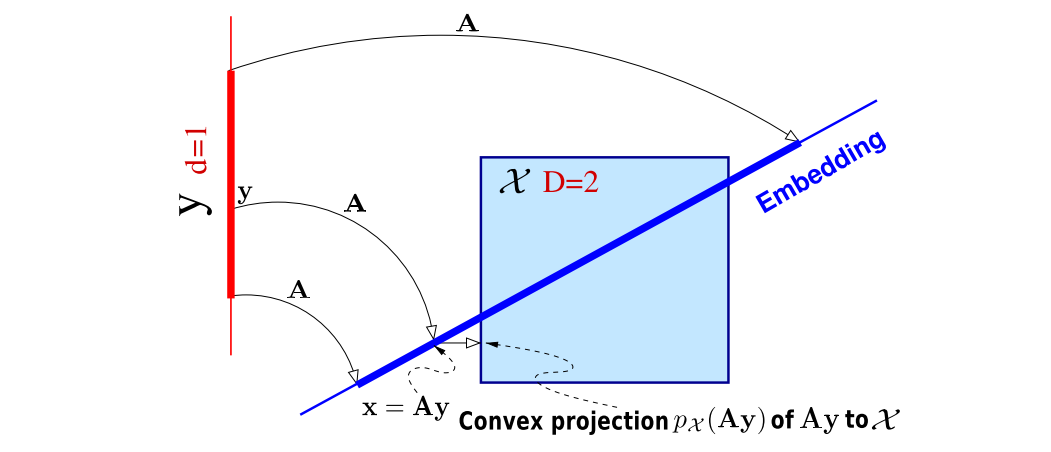
\includegraphics[width=\textwidth]{rembo_convex_projection.png}
        \caption{Parabola Original}
        \label{fig:gull}
    \caption{
    Taken from \citep{Wang2013}: Embedding from $d = 1$ into $D=2$.
    The box illustrates the 2D constrained space $\mathsf{X}$, while the thicker red line illustrates the 1D constrained space $\mathsf{Y}$.
    Note that if $Ay$ is outside $\mathsf{X}$, it is projected onto $\mathsf{X}$.
    The set $\mathsf{Y}$ must be chosen large enough so that the projection of its image, $A\mathsf{Y}$, onto the effective subspace (vertical axis in this diagram) covers the vertical side of the box).
    }\label{fig:animals}
\end{figure}

The key point of REMBO is that the matrix $A$ can be chosen as a random orthogonal matrix.
The authors follow with a proof, that if the optimization domain's parameters are well-chosen, that the chance of getting a bad projection matrix has a certain threshold. \\

\cite{Wang}
A function $f : \mathbf{R}^D \rightarrow \mathbf{R}$ is said to have effective dimensionality $d_e$ (where $d_e < D$), if there exists a linear subspace $\mathcal{T}$ of dimension $d_e$ such that for all $ x_\top \in \mathcal{T} \subset \mathbf{R}^D $ and $x_\perp \in \mathcal{T_\perp} \subset \mathbf{R}^D $, we have $ f(x) = f(x_\top +x_\perp ) = f(x_\top)$.
$\mathcal{T^\perp}$ is the orthogonal complement of $\mathcal{T}$.

Assume $ f : \mathbf{R}^D \rightarrow \mathbf{R} $ has effective dimensionality $d_e$.
Given a random matrix $ \mathbf{A} \in \mathbf{R}^{D \times d} $ (where $d \geq d_e$) with independent entries sampled from $ \mathcal{N}(0, 1) $.
For any $ x \in \mathbf{R}^D $, there exists a $y \in \mathbf{R}^d $ such that $ f(x) = f(\mathbf{A} y ) $.
We now only need to optimize over all possible $y \in \mathbf{R}^d$, instead of all possible $x \in \mathbf{R}^D $. \\


\begin{figure}[H]
    \centering
        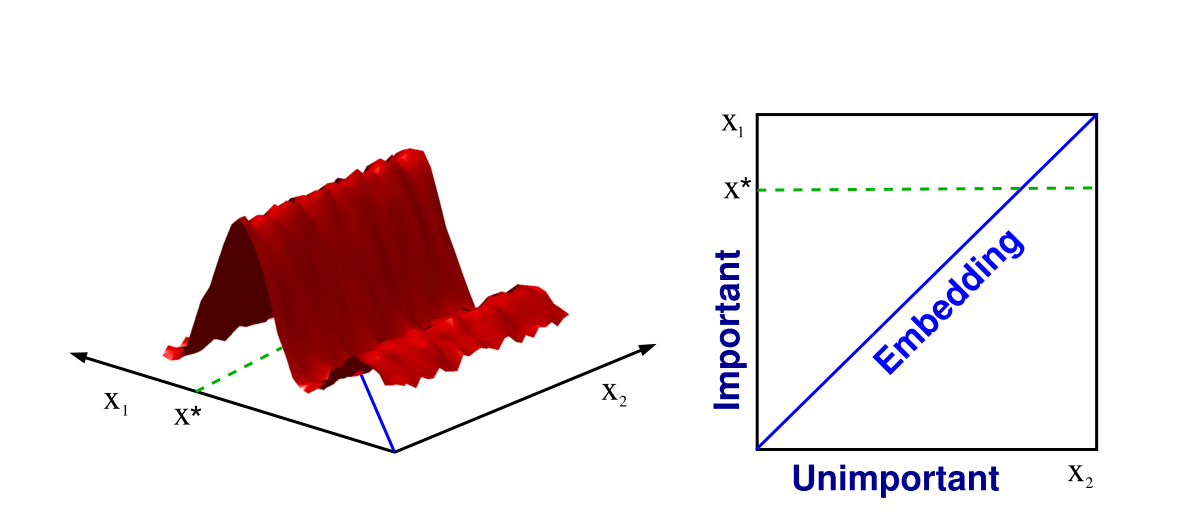
\includegraphics[width=\textwidth]{rembo_sinus_function.png}
        \caption{Parabola Original}
        \label{fig:gull}
    \caption{
    Taken from \citep{Wang2013} Fig. 2: This function in D=2 dimesions only has d=1 effective dimension: the vertical axis indicated with the word important on the right hand side figure. 
    Hence, the 1-dimensional embedding includes the 2-dimensional function’s optimizer. 
    It is more efficient to search for the optimum along the 1-dimensional random embedding than in the original 2-dimensional space.
    }\label{fig:animals}
\end{figure}

Because the authors point at being able to decrease this threshold, they propose interlaved runs, where for each fifth point selection, a differently sampled orthogonal random matrix is chosen. \\

Extensions to REMBO include \citep{RemboExtension}.

\subsection{Applications to high-dimensional uncertainty propogation}
Because the algorithm we propose uses this method to identify the subspace projection matrix, I will discuss this algorithm in more detail.

\citep{Tripathy} This algorithm assumes that  $f(x) \sim g( \mathbf{W}^T y)$ where $ \mathbf{W} \in \mathbb{R}^{D \times d} $ and $D >> d$.
$ \mathbf{W} $ is orthogonal. \\

This algorithm does not require gradient-information.
This makes it easier to implement, and more robust to noise according to the authors of this paper. \\
The GP nosie variance, kernel parameters and  $ \mathbf{W} $ can be found iteratively.
The main idea of the algorithm is to fix the kernel parameters and the GP nosie variance, and identify $ \mathbf{W} $.
Then, we fix $ \mathbf{W} $ and train over the kernel parameters and the GP nosie variance.
This procedure is repeated until the change of the log-likelihood between iterations is below some $ \epsilon_l $, or if the maximum number of steps of optimization is reached.
We repeat this procedure .\\

\paragraph{I now proceed with a more detailed description of the algorithm.}
The quantities of interest are

\begin{align}
\mu_f &= \int f(x) p(x) dx \\
\sigma^2_f &= \int ( f(x) - \mu_f )^2 p(x) dx \\
f \sim p(f) &= \int \delta( f - f(x) ) p(x) dx
\end{align}

The authors argue that w.l.o.g., one can regard only on orthogonal matrices, as this does not restrict the search space of projection matrices, the main reason being that no projection subspace is neglected by doing this.
Here, the family of orthogonal matrices of dimension $d \times D$ is denoted by $\mathbf{W} \in V_d(\mathbb{R}^D) $.
This quantity is also known as the \textbf{Stiefel manifold} \citep{StiefelBayesianInference} \citep{StatisticsStiefelIntro} \citep{StiefelNonparametric}, where $d$ is the found effective dimension of the function, and $D$ is the real input dimension to the function. \\

\subsubsection{Kernel used}
As in the paper, I use the Matern-32 kernel function.
This function has two input vectors $a$ and $b$.

\begin{align}
K(a,  b, \theta) = s^2 \left( 1 + \sqrt{3} \sum_{i=1}^l \frac{(a_i - b_i)^2}{ \textit{l}_i} \right) exp\left( - \sqrt{3} \sum_{i=1}^l \frac{(a_i - b_i)^2}{ \textit{l}_i} \right)
\end{align}

Because I want to avoid numerical testing and implementation, I use the derivative as provided in the GPy library.
The $s, l_1, \ldots, l_l $ are hyper-parameters of the kernel. 
The concatenated vector of all these kernel hyperparameters is denoted by $\theta$. \\

The only modification made to this kernel is the additional parameter $W$:

\begin{equation}
k_{AS} : \mathbb{R}^D \times \mathbb{R}^D \times V_d(\mathbb{R}^D) \times \phi -> \mathbb{R} \\
\end{equation}
\text{where the kernel has the form}
\begin{equation}
k_{AS} (x, x'; W, \phi) = k_d(W^T x, W^T x'; \phi)
\end{equation}


\subsubsection{Step 1.: Determine the active projection matrix W}.
In this step, the algorithm optimizes $W \in V_d(\mathbb{R}^D)$ while keeping the kernel hyperparameters $\phi$ and the GP noise variance $s_n$ fixed.

To simplify calculations later, we define the function, where all parameters but $W$ are fixed as $F$. 
The other parameters are determined from previous runs, or are freshly sampled:

\begin{align}
F(W) &:= \mathcal{L}(W, s_n; X, y) \\
& = \log p(y | X, W, s_n) \\
& =  -\frac{1}{2} (y - m)^T (K + s_n^2 I_N)^{-1} (y - m) -\frac{1}{2} \log|K + s_n^2 I_N| -\frac{N}{2} \log 2 \pi   \\
\end{align}

where $\phi, s_n; X, y$ are fixed and $m$ is the prior mean function, which is 0 in our specific case.

To optimize over the loss function, the algorithm defines the derivative of $F$ with regards to each individual element of the weights-matrix:

\begin{align}
\nabla_{w_{i,j}} F(W) &:= \nabla_{w_{i,j}} \mathcal{L}(W, s_n; X, y) \\
& = \frac{1}{2} \text{tr} \left[ \{ (K + s_n^2 I_N)^{-1} (y-m) \left( (K + s_n^2 I_N)^{-1} (y-m) \right)^T - (K + s_n^2 I_N)^{-1} \} \nabla_{w_{i,j}} (K + s_n^2 I_N) \right]
\end{align}

both these functions depend on the kernel $K$, and it's derivative $\nabla_{w_{i,j}} K$. \\

To optimize over $F$, a more sophisticated algorithm is used, that resembles iterative hill-climbing algorithms.
First, the paper defines the function whose output is a matrix in the Stiefel manifold

\begin{equation}
\gamma(\tau; W) = (I_D - \frac{\tau}{2} A(W) )^{-1} (I_D + \frac{\tau}{2} A(W) ) W
\end{equation}


where $W$ is a fix parameter, and $\tau$ is the variable which modifies the direction that we move on in the Stiefel manifold and with

\begin{equation}
A(W) = \nabla_{W} F(W) W - W ( \nabla_{W} F(W) )^T
\end{equation}

One iteratively chooses fixed $W$, and does a grid-search over $\tau$ such that at each step, the log-likelihood $\mathcal{L}$ is increased.

\subsubsection{Step 2.: Optimizing over GP noise variance and the kernel hyperparameters}

We determine the hyperparameters by optimizing over the following loss function, where $X$ are the input values, $Y$ are the corresponding output samples. $\phi$ is the concatenated vector of the kernel hyperparameters and the GP noise variance. \\

One keeps the $W$ fixed (either by taking $W$ from the last iteration, or freshly sampling it), and then defines the loss function

\begin{equation}
	L(\phi) = \mathcal{L}(W, \phi, \sigma_n; X, y) 
\end{equation}

To optimize this loss function, a simple optimization algorithm such as $L-BFGS$ is used to individually maximize each element of the hyperparameter vector with regards to the log-likelihood.
This is done for a maximum number of steps, or until the change of improvement becomes marginal. \\

\subsubsection{Additional details}
Because initialization is a major factor in this algorithm, these steps are iteratively applied for many hundred steps.
There are also many tens or hundreds of restarts to ensure that the search on the Stiefel manifold results in a good local optimum, and does not get stuck on a flat region with no improvement.
This algorithm is very sensitive on the initially sampled parameter $W$.

\subsubsection{Identification of active subspace dimension }
One cannot know the real active dimension of a problem that one does not know the solution to.
As such, the proposed to apply the above algorithms iteratively by increasing the selected active dimension $d$.
The moment where the relative change between the best found matrix between two iterations is below a relative threshold $\epsilon_s$, the previous active dimension is chosen as the real active dimension. 
The algorithm identifies the loss for each possible active dimension.
It then chooses a dimension, where the relative difference to the previous loss (of the one-lower dimension) is below a certain threshold.

\section{Algorithms that exploit additive substructures}

Functions with additive substructures can be decomposed into a summation over subfunctions, such that
$ f(x) \sim g_0(x) + g_1(x) + \ldots g_2(x) $ where each $g_i$ may operate only on a subset of dimensions of $x$.

\subsection{Independent additive structures within the target function}
% TODO: work on this algorithm a little more extensively, such that you can show the intuition, and potentially a short algorithm outline

\citep{Gardner2017} Assume that $f(x) = \sum_{i=1}^{ |P| } f_i (x[P_i] )$, i.e. $f$ is fully additive, and can be represented as a sum of smaller-dimensional functions $f_i$, each of which accepts a subset of the input-variables.
The kernel also results in an additive structure: $f(x) = \sum_{i=1}^{ |P| } k_i (x[P_i], x[P_i])$.
The posterior is calculated using the Metropolis Hastings algorithm.
The two actions for the sampling algorithm are 'Merge two subsets', and 'Split one set into two subsets'.
$k$ models are sampled, and we respectively approximate $p(f_* | D, x^*) = \frac{1}{k} \sum_{j=1}^{k} p( f(x^* | D, x, M_j) )$, where $M_j$ denotes the partition amongst all input-variables of the original function $f$.

\section{Additional approaches}

\subsection{Elastic Gaussian Processes}
% TODO: Shortly touch on this, give an intuition, but nothing more

\citep{Rana2017} Use a process where the space is iteratively explored.
The key insight here is that with low length-scales, the acquisition function is extremely flat, but with higher length-scales, the acquisition function starts to have significant gradients.
The two key-steps is to 1.) additively increase the length-scale for the gaussian process if the length-scale is not maximal and if $|| x_{init} - x^* || = 0$.
And 2.) exponentially decrease the length-scale for the gaussian process if the length-scale is below the optimum length-scale and if $|| x_{init} - x^* || = 0$.


\subsection{Bayesian Optimization using Dropout}
% TODO: Shortly touch on this, give an intuition, but nothing more

\citep{Li2018} propose that the assumption of an active subspace is restrictive and often not fulfilled in real-world applications.
They propose three algorithms, to iteratively optimize amongst certain dimensions that are not within the $d$ 'most influential' dimensions: 1.) Dropout Random, which picks dimensions to be optimized at random, 2.) Dropout copy, which continuous optimizing the function values from the found local optimum configuration, and 3.) which does method 1. with probability $p$, and else method 2.
The $d$ 'most influential' dimensions are picked at random at each iteration. \\

Additional works I explored as background research or additional methods include \citep{KernelGibbsSampler}, \citep{VirtualVsReal}, \citep{SensorPlacement}, \citep{BatchedBO}, \citep{GPforML}.
%% IMPLEMENTATION

\chapter{Model Design and Training} 
\label{ch4}

This chapter gives the detail of the model structure, including the vocabulary encoding, network architecture, regularisation and training procedure. At a high-level, the model's architecture is based on Mikolov's skip-gram model, augmented with additional embeddings at the input layer such that the model is now sensitive to user contexts; hence the model presented in this thesis is called the \ti{Context-dependent skip-gram} (CDSG).

\section{Model}

\tb{Hierarchical softmax}

The original neural probabilistic language model as presented by Bengio \ti{et al.} suffers from a highly inefficient softmax normalisation at the output layer (see Equation~\ref{eq:ch2:output_layer}), as the final conditional probabilities are normalised over $|V|$ different possible words and the size of the vocabulary makes the computation impractical (often $10^5$--$10^7$ terms).
\nl
Several workarounds have been suggested for this problem, one of which is known as the \ti{hierarchical softmax} developed by Morin and Bengio~\cite{morin05}. Hierarchical softmax is a computationally efficient approximation to the full softmax, where a binary tree is built with all $|V|$ words in the vocabulary as the leaf nodes. The inner nodes denote some semantic grouping of their child nodes. Given a binary representation $(b_m(w), b_{m-1}(w), \dots, b_1(w))$ of a word $w \in V$ , where $b_j(w)$ denotes the j\textsuperscript{th} node on the path from the root to the leaf node $w$, the conditional probability of the next word can be approximated as:
\begin{equation}
P(w|w_{t-1},\dots,w_{t-n+1}) = \prod_{j=1}^{m}{P(b_j(w)|b_{j-1}(w),\dots,b_1(w),w_{t-1},\dots,w_{t-n+1})}.
\label{eq:ch4:bengio_softmax}
\end{equation}
By keeping the binary tree balanced, this structure provides an exponential speed-up, on the order of $\frac{|V|}{\log_2{|V|}}.$ Note that we now need to maintain an \ti{additional embedding matrix} for all nodes in the binary tree. In Equation~\ref{eq:ch4:bengio_softmax}, $w,w_{t-1},\dots,w_{t-n+1}$ are standard word embedding vectors, whereas $b_j(w),b_{j-1}(w),\dots,b_1(w)$ are individual bits of Huffman node embeddings, explained further in the next section.
\nl
In their paper introducing negative sampling, Mikolov \ti{et al}. give the following formulation for hierarchical softmax in the skip-gram model~\cite{mikolov13b}. Standard softmax output in the skip-gram model defines $p(w_{t+j}|w_t)$ as:
\begin{equation}
p(w_O|w_I) = \frac{\exp({v'_{w_O}}^{\intercal}v_{w_I})}{\sum_{w=1}^{|V|}\exp({v'_{w}}^{\intercal}v_{w_I})},
\label{eq:ch4:skip_softmax}
\end{equation}
where $v_w$ and $v'_w$ are standard embeddings and Huffman node embedding of $w$, respectively. The dot product ${v'_{w_O}}^{\intercal}v_{w_I}$ gives a measure of `similarity' between the target and the context word. The intuition is that the higher the similarity is, the more weight the target word receives during prediction. 

In a binary tree vocabulary where each word $w$ can be reached by some path from the root, let $n(w,j)$ be the $j$-th node on the path from root to $w$. Also let $L(w)$ be the length of the path to $w$. Hence, $n(w,1)=root$ and $n(w,L(w))=w$. For any inner node $n$, let $ch(n)$ be the left child of node $n$. Then, the conditional probability can be given as:
\begin{equation}
P(w|w_I)=\prod_{j=1}^{L(w)-1}{\sigma([\![n(w,j+1)=ch(n(w,j))]\!]\cdot {v'_{n(w,j)}}^{\intercal} v_{w_I} )},
\label{eq:ch4:morin}
\end{equation}
where $\sigma(x)=\frac{1}{1+\exp(-x)}$ and $[\![x]\!]=1$ if $x$ is true and $-1$ if otherwise. $v_{w_I}$ and ${v'_{n(w,j)}}$ are standard embedding of the input word and Huffman embedding of the $j$-th node on the path to the output word. Similarly to Equation~\ref{eq:ch4:skip_softmax}, the dot product represents a measure of similarity between the input and output word, with the output word decomposed into several layers of clusters, each making different contributions to the semantic representation of the output word.
\nl
The sigmoid function $\sigma$ acts as a normalisation technique, as $\sigma(x)+\sigma(-x)=1$. Hence, for a given inner node $w_1$ with child nodes $w_2$ and $w_3$, $\sigma(w_2|w_1) + \sigma(w_3|w_1)=1$, therefore all transition probabilities for every node in each level in the tree sum to 1.

\begin{figure}
	\vspace{-20mm}
	\hspace{-10mm}
        \begin{subfigure}[b]{8cm}
                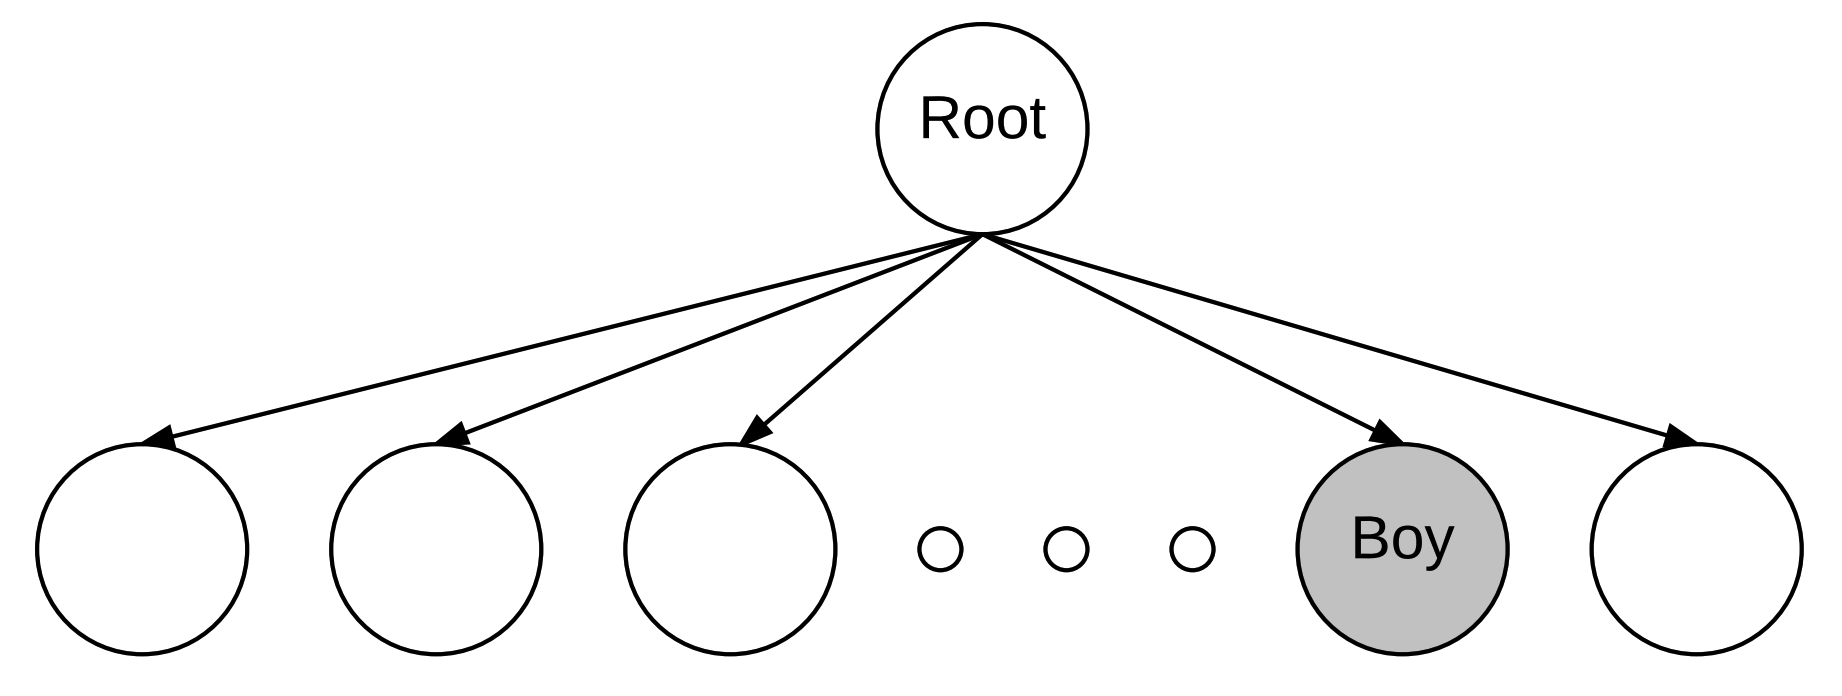
\includegraphics[width=8cm]{figs/chap4/original_nnlm.png}
		\captionsetup{justification=centering}
                \caption{Original vocabulary as flat list.\\ \color{white}{ here's the hid}}
                \label{fig:chap4:original_nnlm}
        \end{subfigure}%
        ~ %add desired spacing between images, e. g. ~, \quad, \qquad, \hfill etc.
          %(or a blank line to force the subfigure onto a new line)
        \begin{subfigure}[b]{7cm}
                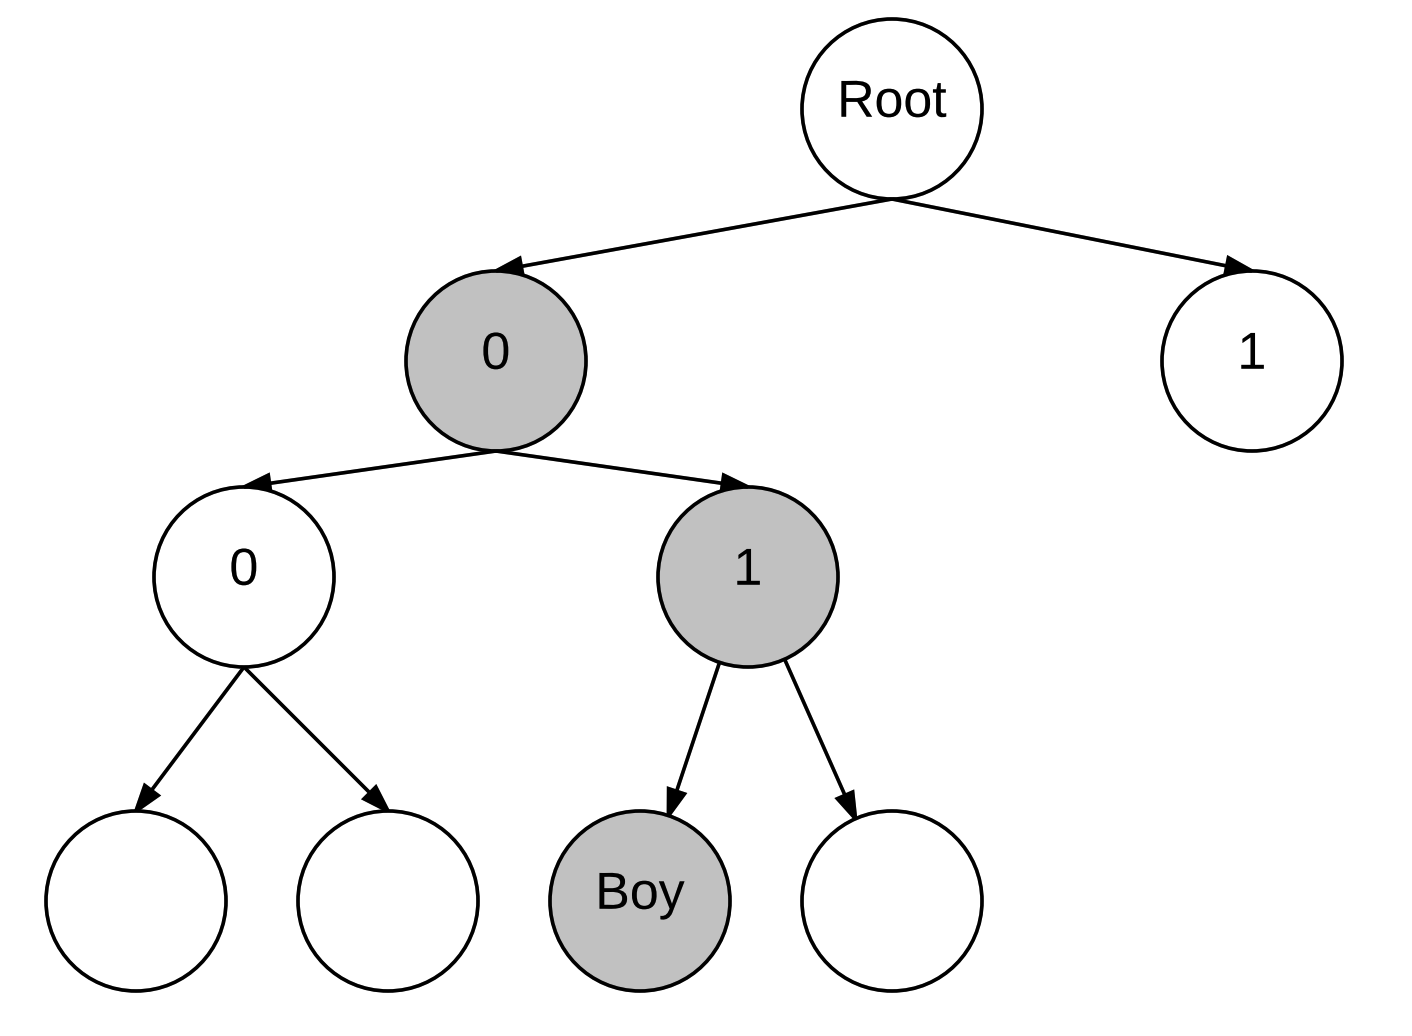
\includegraphics[width=7cm]{figs/chap4/hierarchical.png}
                \captionsetup{justification=centering}
                \caption{Binary tree vocabulary with hierarchical softmax.}
                \label{fig:chap4:hierarchical}
        \end{subfigure}
	\captionsetup{justification=centering}
        \caption[Vocabulary structures.]{Vocabulary structures of orignal neural network language model and hierarchical sampling.}
        \label{fig:chap4:vocab}
\end{figure}        

\tb{Vocabulary}

For the binary encoding of words, an optimal prefix code known as the Huffman encoding scheme was chosen~\cite{huffman52}. Constructing a Huffman binary tree starts by sorting all words by their frequency, making the two least frequent words into leaf nodes. Then their parent node is created with the sum of its children's frequencies as its frequency. Excluding the two leaves (but including their parent node), two least frequent words are again selected, and the process is repeated until a single root note remains with the sum of every word's frequency. 
\nl
I first constructed a Huffman binary encoding of every vocabulary word, then built a binary tree structure based on the encoding, as in Figure~\ref{fig:chap4:hierarchical}. Then, each bit of the Huffman embedding of a word represents a `left or right' decision in the tree, which when combined in series ultimately forms the semantic representation of the word.

\tb{Network Architecture}

\begin{figure}[htbp]
    \hspace{-2.7cm}
    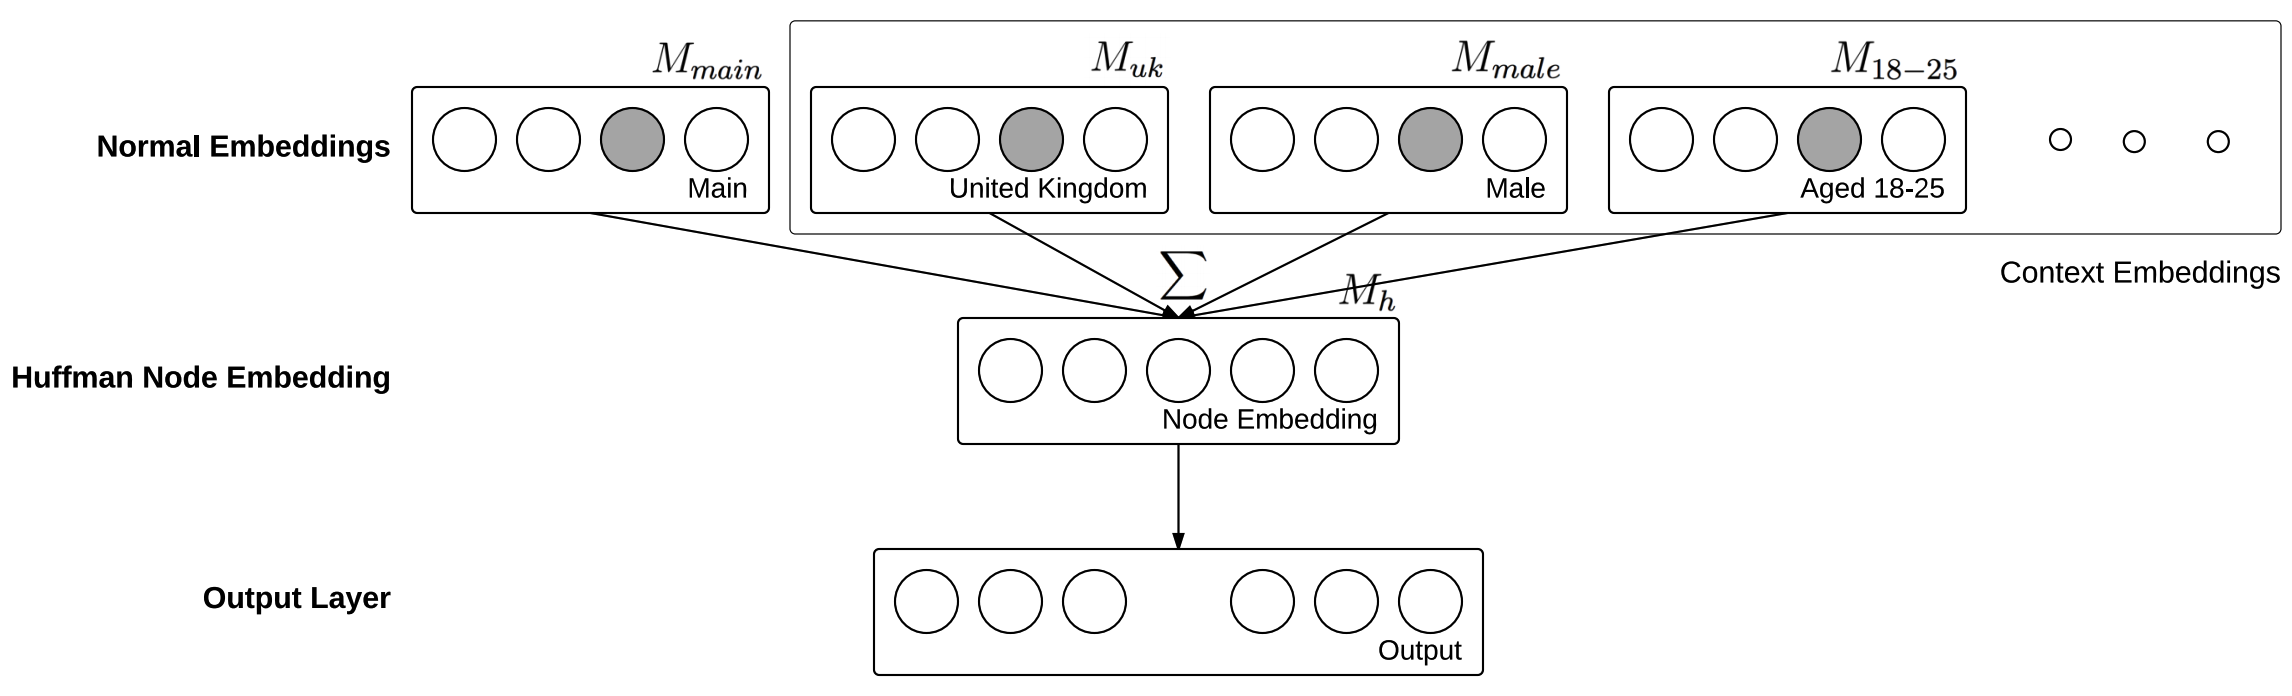
\includegraphics[width=20cm]{figs/chap4/architecture.png}
    \captionsetup{justification=centering}
    \caption[Skip-gram network architecture. ]{Skip-gram network architecture. Given an input words and its contexts, corresponding rows are accessed from the main embedding matrix $M_{main}$ and appropriate context embeddings matrices $M_c$, and summed in the hidden layer.}
    \label{fig:chap4:skipgram}
\end{figure}

Figure~\ref{fig:chap4:skipgram} shows the architecture of the context-dependent skip-gram. It has three sets of parameters (or \ti{weights} in the neural network literature): main word embeddings, context word embeddings and Huffman node embeddings. Main word embedding is a matrix $M_{main} \in \mathbb{R}^{|V|\times k}$ whose $i$-th row contains a $k$-dimensional vector for the $i$-th word in the vocabulary. An embedding for a particular word can be accessed with a \ti{one-hot vector}: $o'=(0,0,0,\dots,1,\dots,0,0,0)^{\intercal} \in \mathbb{R}^{|V|\times 1}$ as $w'={M_{main}}^{\intercal}\;o'\in \mathbb{R}^{k\times 1}.$
\nl
Context embeddings $M_{c}$ are of the same dimension as $M_{main}$ but contain word embeddings particular to a certain user context $c$ that, when combined with the main word embedding, produces final word embeddings for that context. Hence, the embedding of the word \ti{boy} for male in the US is obtained as:
$$w_{boy}'=(M_{main}+M_{male}+M_{us})^{\intercal}\;o_{boy}'$$
The Huffman node embedding matrix $M_{h} \in \mathbb{R}^{Z\times k}$ contains $k$-dimensional embeddings for each inner node in the Huffman vocabulary tree. With input and output words $w_I$ and $w_O$, and a given node level $j$ of the output word, the network computes ${v'_{n(w_O,j)}}^{\intercal}\:v_{w_I}$ as output. Note that $v_{w_I}$ is the embedding for word $w_I$ in the main word embedding matrix $M_{main}$, whereas $v'_{n(w_O,j)}$ is the Huffman node embedding for node $n(w_O,j)$ in the node embedding matrix $M_{h}$.
\refs{HOW MANY CONTEXTS HAVE BEEN CREATED}

\tb{Regularisation}

Hinton \ti{et al.} developed a biologically-inspired regularisation technique to avoid co-adaptation of weights in neural networks~\cite{hinton12}. This technique, known as \ti{Dropout}, randomly omits a hidden unit (sets to zero) from the network with some probability $p$. This is amounts to taking an average of an exponential number of different networks in a very efficient manner, as well as preventing a hidden unit from rely on the presence of any other.
\nl
Dropout was implemented in the CDSG model by randomly excluding some weights during computation of the dot product at the output layer.

\section{Training}

The model was trained using stochastic gradient ascent and backpropagation. Every training example was only fed into the network once and the weights were updated after each example. Only a small number of parameters are updated after the network sees each example: assuming the sentence has contexts \ti{US} and \ti{female}, only two rows of dimension $1\times 200$ in matrices $M_{main}, M_{us}, M_{female}$ and $M_{h}$ are updated for each ($w_I, w_O$) pair.

\tb{Objective function derivation}

The training objective of the model is to find the set of embeddings that maximises the average log probability of the training data:
\begin{equation}
\frac{1}{T}\sum_{t=1}^{T}\sum_{-c \le j \le c, j \ne 0}^{}{\log p(w_{t+j}|w_t)},
\label{eq:ch4:obj}
\end{equation}
where $T$ is the size of the training corpus. Recall that $\log p(w_{t+j}|w_t)$ in the context of skip-gram is given in Equation~\ref{eq:ch4:morin} and repeated below:
\begin{equation}
\prod_{j=1}^{L(w)-1}\sigma([\![n(w,j+1)=ch(n(w,j))]\!]\cdot {v'_{n(w,j)}}^{\intercal} v_{w_I} ).
\label{eq:ch4:sigma}
\end{equation}
Let $sim={v'_{n(w,j)}}^{\intercal} v_{w_I}$ and $code=n(w,j+1)$ (in bits, hence either 0 or 1; 0 represents the left child, while 1 represents the right). Then the expression inside the product can be re-written as:
\begin{equation}
\sigma_{obj}(code,sim)=\frac{\exp((1-code)sim)}{1+\exp(sim)}.
\label{eq:ch4:sol}
\end{equation}
The above holds because in the case where $code=0$ (\ti{i.e.} $j+1$\textsuperscript{th} node is the left child of the $j$-th node):
$$\sigma_{obj}(0,sim)=\frac{\exp(sim)}{1+\exp(sim)}=\frac{1}{1+\exp(-sim)}=\sigma(sim).$$
The expression within $[\![ \cdot]\!]$ in Equation~\ref{eq:ch4:sigma} is true because we choose $ch(n)$ to be the left child of node $n$. Consequently, it evaluates to 1. If, on the other hand, $code=1$:
$$\sigma_{obj}(1,sim)=\frac{1}{1+\exp(sim)}=\sigma(-sim).$$
The expression $[\![ \cdot]\!]$ in this case evaluates to $-1$. Note that $\sigma_{obj}(0,sim)+\sigma_{obj}(1,sim)=1, \: \forall{sim}.$
\nl
Taking the logarithm of Equation~\ref{eq:ch4:sol}, we get
$$\log\sigma_{obj}(code,sim)=(1-code)sim-\log({1+\exp(sim)}).$$
If we take its derivative with respect to $sim$,
\begin{equation}
\begin{split}
\frac{d(\log\sigma_{obj}(code,sim))}{dsim}&=1-code-\frac{\exp(sim)}{1+\exp(sim)} \\ 
									&=1-code-\sigma(sim).
\end{split}
\label{eq:ch4:code}
\end{equation}

As $sim={v'_{n(w,j)}}^{\intercal} v_{w_I}$, where $v'_{n(w,j)}={M_h}^\intercal\:o'_{w_O}$ and $v_{w_I} = (M_{main}+\sum_{c}^{}{M_{c}})^\intercal\:o'_{w_I}$ (where $o'_{w_I}, o'_{w_O}$ are one-hot vector to index into words $w_I$ and $w_O$ respectively), the derivative of $sim$ with respect to each element of the weights are:
\begin{equation}
\frac{dsim}{dM_{main}(i,j)}=\sum_{k}^{}M_{h}(k,j)
\label{eq:ch4:dmain}
\end{equation}
\begin{equation}
\frac{dsim}{dM_{c}(i,j)}=\sum_{k}^{}M_{h}(k,j).
\label{eq:ch4:dc}
\end{equation} assuming $i$ is the index of $w_I$ and $k$ ranges over the indexes of the nodes of $w_O$. $M_{main}(i,j)$ accesses the element of $i$-th row and $j$-th column in matrix $M_{main}$. Also,
\begin{equation}
\frac{dsim}{dM_{h}(k,j)}=(M_{main}+\sum_{c}^{}{M_{c}})(i,j).
\label{eq:ch4:dh}
\end{equation}

\tb{Gradient ascent}

Gradient ascent algorithm increments the parameters with the gradient of the objective function with respect to the parameter, multiplied by the learning rate. This updates the parameters in the direction of the steepest gradient.
$$\theta \leftarrow \theta + \eta\frac{\partial f_{obj}(\theta)}{\partial\theta}.$$ This can be rewritten into 
$$\theta \leftarrow \theta + \eta\frac{\partial sim}{\partial\theta}\:\frac{\partial f_{obj}(sim)}{\partial sim}.$$
Note that the latter partial derivative is given in Equation~\ref{eq:ch4:code}. Hence, this gives
\begin{equation}
\theta \leftarrow \theta + \eta\frac{\partial sim}{\partial\theta}\:(1-code-\sigma(sim)).
\label{eq:ch4:grad}
\end{equation}
Letting $\theta=M_{z}(i,j)$ where $z \in \{main,c,h\}$ , the appropriate gradient $\frac{\partial sim}{\partial M_z(i,j)}$ is given in \cref{eq:ch4:dmain,eq:ch4:dc,eq:ch4:dh}.

\tb{Backpropagation}

Standard backpropagation is performed to update the weights of the network. In forward propagation, a single row in $M_{main}$ and $M_{c}$ interacts with multiple rows in $M_h$, as the output word is decomposed into several nodes. Hence, the gradient of $M_{main}$ and $M_c$ is accumulated over all nodes on the path to the output word and updated at the end. On the other hand, each row of $M_h$ interacts only with one row of $M_{main}$ and each of $M_c$, hence can be updated immediately.

\vspace{5pt}
\begin{algorithm}[htbp]
\begin{description}
	\item For each inner node along to path to the output word $w_O$:
		\item \quad Compute a forward pass through the network, obtain $1-code-\sigma(sim).$
		\item \quad Update $M_{h}$ with the gradient of $M_h$: sum of relevant rows in $M_{main}$ and $M_c$.
		\item \quad Accumulate gradients of $M_{main}$ and $M_c$.		
	\item Update $M_{main}$ and $M_c$ with the accumulated gradient.
\end{description}
\caption{Outline of training process.}
\label{alg:chap4:backprop}
\end{algorithm}

\tb{Context-specific learning rate}

Mikolov's implementation uses a single global learning rate that linearly decays from an initial value. All weights in $M_{main}$ and $M_h$ are updated with the same learning rate. 
\nl
For the context-dependent skip-gram, given that examples with different contexts appear with different frequencies in the training data, it makes sense to have a separate learning rate for each context $c$. This enables the network to learn relatively little from a single example of frequently occurring contexts, and to pay more attention to examples with rare and informative contexts, thereby learning more from those occurrences.
\nl
The learning rate $\eta(c,t)$ for the context $c$ at time $t$ during training evolves as:
$$ \eta(c,t) = \max(\eta_{min}, \eta_0 \times(1-\frac{\delta_t(c)}{\delta_{total}(c)})).$$
$\eta_{min}, \eta_0$ are predefined values for initial and final learning rates (shared by all contexts). $\delta_t(c)$ is the number of words associated with context $c$ seen so far up to time $t$ during training, and $\delta_{total}(c)$ is the total number of words tagged with context $c$ in the training corpus. Empirically, $\eta_{min}, \eta_0$ were chosen as $0.0001$ and $0.1$.

\section{Implementation}

\tb{Cython}

Rehurek's implementation was optimised for selected hotspots by calling core C routines and BLAS functions within Cython code. As Cython's memory management is not thread-safe, implementing training and dropout in Cython involved careful use of global mutex called GIL (Global Interpreter Lock) to prevent several threads from accessing Python bytecodes simultaneously.

\vspace{0.3cm}
\begin{lstlisting}[language=Python,caption={Cython code for dropout regularisation at the hidden layer.},label=lst:chap4:dropout]
for a in range(0, size):
    syntemp[a] = syn0[indexes[j] * size + a]

# Summing context embeddings 
for x in range(0, context_length):
    for a in range(0, size):
        syntemp[a] += syncon[ (contexts[x]*vocab_size*size)
        						 + indexes[j] * size + a ]

# Dropout
for a in range(0, size):
    if (xor32() % 100) < dropout_param:
        syntemp[a] = 0
\end{lstlisting}

Listing~\ref{lst:chap4:dropout} shows a Cython code snippet to implement summation of main and context word embeddings at the input layer and drop hidden units out with some probability afterwards.

\tb{BLAS functions}

BLAS (Basic Libear Algebra Subprograms) is a set of interfaces to perform linear algebra operations with heavy optimisations in C and Fortran. As several operations in the backpropagation routine involve computing the dot product of vectors, BLAS functions were used to optimise a loop of similar linear algebra operations. An example is the \tx{dsdot(n,x,incx,y,incy)} function, which computes the dot product of vectors \tx{x} and \tx{y} of size \tx{n}, with increment \tx{incx} and \tx{incy} to index each element of the vectors.

\tb{Precomputed sigmoid table}\footnote{Optimisation used by Mikolov \ti{et al.} in the C implementation: \url{https://code.google.com/p/word2vec/source/browse/trunk/word2vec.c}.}

As Equation~\ref{eq:ch4:grad} shows, computing the gradient involves obtaining $\sigma(sim)$. As evaluating the sigmoid function on every training example can lead to a significant performance hold-up, the sigmoid function was precomputed in discretised steps and stored in a table, effectively replacing explicit sigmoid evaluations in the core training routine with dictionary lookups.

\begin{lstlisting}[language=Python,caption={Cython code for precomputing and accessing sigmoid function.},label=lst:chap4:sigmoid]
# computing the sigmoid table.
for i in range(SIG_TABLE_SIZE):
	SIG_TABLE[i] = exp((i / SIG_TABLE_SIZE * 2 - 1) * MAX_SIG)
	SIG_TABLE[i] = (SIG_TABLE[i] / (SIG_TABLE[i] + 1))

# f is the vector similarity (dot product)
if f <= -MAX_SIG or f >= MAX_SIG:
	continue
f = SIG_TABLE[((f + MAX_SIG) * (SIG_TABLE_SIZE / MAX_SIG / 2))]
\end{lstlisting}

\begin{figure}[htbp]
%   \vspace{-1.5cm}
   \centering
    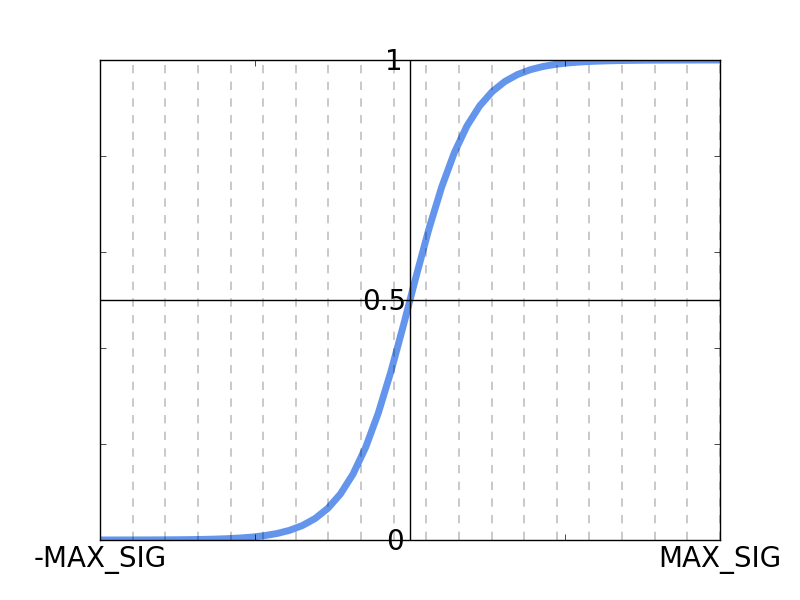
\includegraphics[width=9cm]{figs/chap4/sigmoid.png}
    \captionsetup{justification=centering}
    \caption[Discretisation of the sigmoid function. ]{The sigmoid function is discretised into \tx{SIG\_TABLE\_SIZE} pieces.}
    \label{fig:chap4:sigmoid}
%    \vspace{-1cm}
\end{figure}

In Figure~\ref{fig:chap4:sigmoid}, note that $\sigma(x)\approx 1$ if $x$ is large and $\sigma(x)\approx 0$ if $x$ is small. Hence we define a boundary \tx{MAX\_SIG} such that we approximate the function as 0 and 1 if $x$ is beyond either barrier. Within that range, we discretise the function into \tx{SIG\_TABLE\_SIZE} pieces. Concretely, \tx{MAX\_SIG} and \tx{SIG\_TABLE\_SIZE} were chosen to be 6 and 1000, respectively. 
\nl
In Listing~\ref{lst:chap4:sigmoid}, \tx{SIG\_TABLE} is defined as:
\begin{equation}
\begin{split}
\tx{SIG\_TABLE[i]} &= \frac{ \exp((\frac{2*i}{\tx{SIG\_TABLE\_SIZE}} - 1) * \tx{MAX\_SIG}) }{\exp((\frac{2*i}{\tx{SIG\_TABLE\_SIZE}}  - 1) * \tx{MAX\_SIG}) + 1} \\
				&= \frac{1}{1+\exp(-(\frac{2*\tx{MAX\_SIG}}{\tx{SIG\_TABLE\_SIZE}}*i - \tx{MAX\_SIG}) )}
\end{split}
\end{equation}

Then, 
%\begin{multline}
$$\tx{SIG\_TABLE}[((f + \tx{MAX\_SIG}) * \frac{\tx{SIG\_TABLE\_SIZE}}{\tx{MAX\_SIG}*2})] $$
\begin{equation}
\begin{split}
&= \frac{1}{1+\exp(-(\frac{2*\tx{MAX\_SIG}}{\tx{SIG\_TABLE\_SIZE}}*((f + \tx{MAX\_SIG}) * \frac{\tx{SIG\_TABLE\_SIZE}}{\tx{MAX\_SIG}*2}) - \tx{MAX\_SIG}) )} \\
&= \frac{1}{1+\exp(-((f + \tx{MAX\_SIG}) - \tx{MAX\_SIG}) )} \\
&= \frac{1}{1+\exp(-f)} \\
&= \sigma(f)
\end{split}
\end{equation}
%\end{multline}

Hence, this method correctly computes the value of the sigmoid function.

\tb{Shuffling tweets}

As that the learning rate decreases linearly throughout training, the network learns the most from examples that appear early in the training corpus. Therefore, shuffling the order of the tweets causes huge perturbations on the evolution of the cost function of the network, thereby allowing the model to explore different regions of the cost surface throughout several iterations of training. When training the same model several times to obtain the performance bound, the examples were shuffled by random for each training session. This leads to a more robust evaluation of the model's performance independently of the order of samples. 

\tb{Initialising embeddings}

Mikolov's implementation of Skip-gram initialises each element of the general embedding matrix with a random draw from a uniform distribution $[-0.5, 0.5].$ This is the only source of randomness in the original C implementation. However, I chose to initialise the general embeddings with an external embedding matrix pre-learnt from a standard corpus such as Wikipedia. This will potentially lead to performance improvements because the model now has substantial knowledge about facts from Wikipedia. For example, it can now learn more nuanced changes in meaning of `Mercedes' in different contexts as it already knows that Mercedes is a carmaker. 
\nl 
As such, I trained the standard Skip-gram model on the first billion characters from Wikipedia\footnote{\url{http://mattmahoney.net/dc/enwik9.zip}}. Then, I initialised the general embeddings of words in my model with the embeddings learnt from Wikipedia. The words in my model that do not occur in Wikipedia were simply initialised as before: uniformly distributed as $[-0.5,0.5].$

\section{Measuring brand perception}

Word association in the vector space model is commonly measured with \ti{cosine similarity} between the two word vectors. Once the context-dependent model is trained, its word embeddings change for different contexts. I propose to measure brand perception as the cosine similarity between word embeddings that represent product category and brand names. For example, to see which of \ti{smirnov, absolut} and \ti{svedka} is most associated with \ti{vodka}, I compute the following:
$$ sim(x,vodka), \: x \in \{smirnov, absolut, svedka\}.$$
$sim(a,b)$ is the cosine similarity between $vec(a)$ and $vec(b)$. The item with the greatest cosine similarity with \ti{vodka} is the one most associated with vodka according to the model's learnt embeddings.
\\ \\
On the other hand, to measure perception with contexts, I can instead compute:
$$ sim_{x}(alcohol,beer), \: x \in \{male, female\},$$
where $sim_{c}(a,b)$ denotes the cosine similarity between $vec(a)$ and $vec(b)$ in the context of $c$. Computing this first involves adding context embeddings for $c$ to the main embeddings of $a$ and $b$, \ti{i.e.}
$$ sim_{c}(a,b) = sim(vec_{main}(a)+vec_c(a),vec_{main}(b)+vec_c(b)).$$
Beer can be said to be more associated with alcohol for one gender if the similarity between $vec(beer)$ and $vec(alcohol)$ is greater in the context of that gender. 

%% EVALUATION

\chapter{Evaluation} 
\label{ch5}

\section{Evaluation setting}

This chapter evaluates the effectiveness of the context-dependent skip-gram model by comparatively assessing the quality of context embeddings against those learnt by a model insensitive to user contexts. Then, it presents notable observations of context embeddings' ability to capture various contextual variations of word meanings.

\tb{Models}

In quantative evaluation schemes (see Section~\ref{ch5:2}), three models were evaluated against each other: 
\begin{itemize}[itemsep=-5pt]
	\item SGLM: Mikolov's vanilla Skip-gram model augmented with context embeddings.
	\item CDSG: SGLM model with context-specific learning rates.
	\item CDSGD: CDSG model with 10\% of its hidden units randomly omitted with dropout. 10\% was found to give best performance.
\end{itemize}

\tb{Parameter set}

The list of model-generic parameters and the values used in practice are given below:

\begin{itemize}[itemsep=-5pt]
	\item vector\_size : the dimension of the learned vector representations, chosen to be 200.
	\item ini\_alpha : initial learning rate (both general and context-specific), chosen to be 0.1. 
	\item min\_alpha : minimum learning rate (both general and context-specific), chosen to be 0.0001.
	\item window : the width of the context-window from which to perform word prediction, chosen to be 5. This implies that all contexts within five words to the left and the right were used to predict the current word.
	\item min\_count : the threshold for which words appearing in corpus with a smaller frequency are ommitted, chosen as 50.
\end{itemize}

\section{Quantitative evaluation}
\label{ch5:2}

As a quantitative measure of the model's ability to learn context-sensitive representations of language, I constructed three different evaluation schemes, which each test if the model captures different types of metadata well.

\subsection{Location}

\tb{Dataset and methodology}

To evaluate the accuracy of geographic embeddings, I adopted the dataset used by Bamman \ti{et al.} to evaluate distributed representations to learn geographically situated language~\cite{bamman14}. The authors measure semantic similarity of pairs of words whose meaning has strong geographic correlations and report the mean similarity of geographically-related pairs of words. For example, in U.S., California, we expect the word \ti{state} to be associated most with \ti{california} than any other American state, such as \ti{texas}. I take the rank of \ti{california} from all states based on the similarity to vector \ti{state} in the context of \ti{california}, and proceed with other states analogously. Six categories of words with strong geographic connotation were constructed, as shown below. For each category, an example of the list of similarities to be computed is shown for each sports team/state, with the target similarity (the one we expect to rank highest) displayed in bold.

\begin{enumerate}[itemsep=-15pt]
	\item \tb{state}: for each state, I compute the similarity between the word \ti{state} and every US state, in the context of that state; \\ \ti{e.g.}, $\mathbf{sim_{CA}(state,california)},sim_{CA}(state, texas),sim_{CA}(state, arizona),\\ \cdots$ for the state California.
	\item \tb{city}: for each state, I compute thet similarity between the word \ti{city} and the most populous city of each state, in the context of that state; \ti{e.g.}, $\mathbf{sim_{MA}(city,boston)},sim_{MA}(city,new\:york), sim_{MA}(city,houston),\\ \cdots$ for the state Massachusetts. 
	\item \tb{basketball}: for each NBA team, I compute the similarity between $(vec(basketball)+vec(team))$ and every NBA team name, in the context of the state the team is based in; \\ \ti{e.g.} $\mathbf{sim_{IL}(basketball+team,bulls)},sim_{IL}(basketball+team,knicks),\\sim_{IL}(basketball+team,celtics), \cdots$ for the team Chicago Bulls
	\item \tb{baseball}: for each MLB team, I compute the similarity between \\ $(vec(baseball)+vec(team))$ and every MLB team name, in the context of the state the team is based in; \\ \ti{e.g.} $\mathbf{sim_{MA}(baseball+team,red\:sox)},sim_{MA}(baseball+team,yankees),\\sim_{MA}(baseball+team,white\:sox),\cdots$ for the team Boston Red Sox. 
	\item \tb{football}: for each NFL team, I compute the similarity between \\ $(vec(football)+vec(team))$ and every NFL team name, in the context of the state the team is based in; \\ \ti{e.g.} $\mathbf{sim_{TX}(football+team,cowboys)},sim_{TX}(football+team,giants),\\ sim_{TX}(football+team,bears),\cdots$ for the team Dallas Cowboys.
	\item \tb{hockey}: for each NHL team, I compute the similarity between \\ $(vec(hockey)+vec(team))$ and every NHL team name, in the context of the state the team is based in;\\  \ti{e.g.} $\mathbf{sim_{NJ}(hockey+team,devils)},sim_{NJ}(hockey+team,rangers),\\ sim_{NJ}(hockey+team,islanders),\cdots$ for the team New Jersey Devils.
\end{enumerate}

\begin{figure}[htbp]
	\hspace{-2.3cm}
        \begin{subfigure}[b]{9cm}
                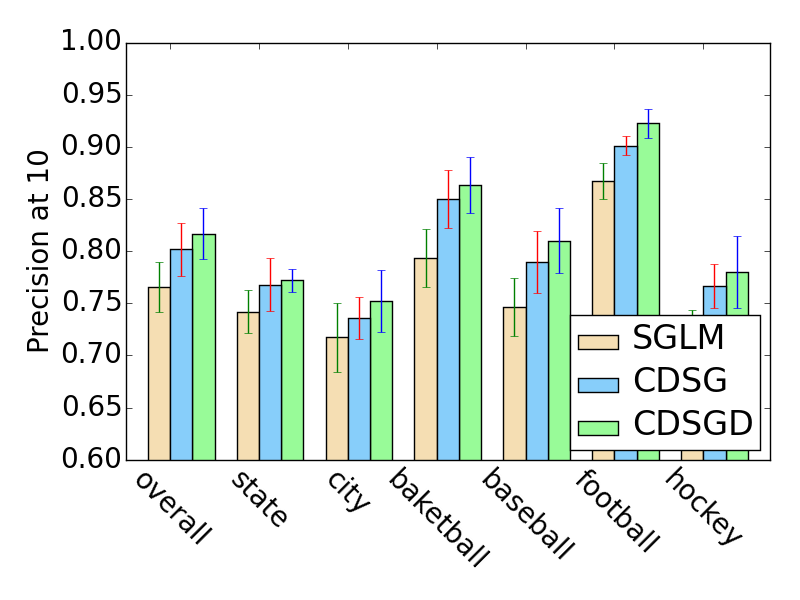
\includegraphics[width=9cm]{figs/chap5/loc_prec.png}
                \caption{Precision at 10 for each category}
                \label{fig:chap5:loc_prec}
        \end{subfigure}%
        ~ %add desired spacing between images, e. g. ~, \quad, \qquad, \hfill etc.
          %(or a blank line to force the subfigure onto a new line)
        \begin{subfigure}[b]{9cm}
                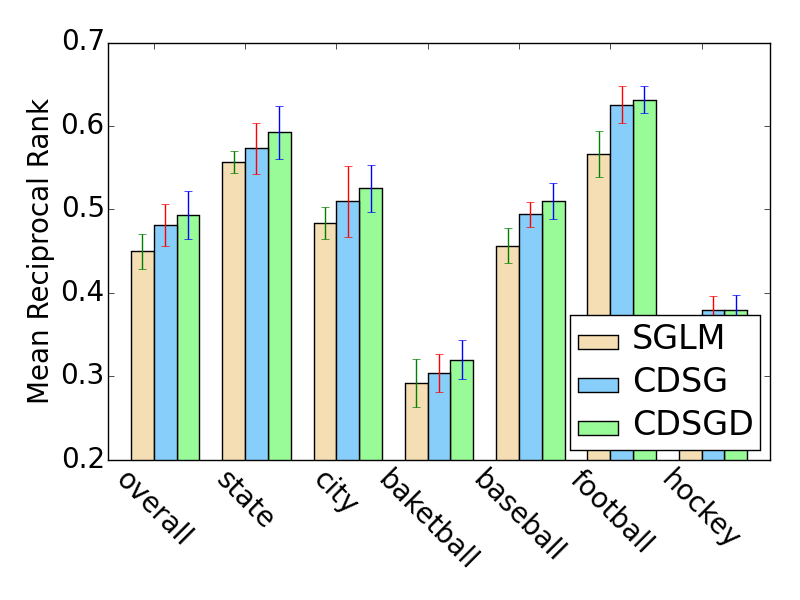
\includegraphics[width=9cm]{figs/chap5/loc_mrr.png}
                \caption{Mean reciprocal rank for each category.}
                \label{fig:chap5:loc_mrr}
        \end{subfigure}
	\captionsetup{justification=centering}
        \caption[Location evaluation results.]{Location evaluation results.}
        \label{fig:chap5:loc_eval}
\end{figure}

Three models (SGLM, CDSG, CDSGS) were each run five times with the same parameter set and the training data shuffled. In Figure~\ref{fig:chap5:loc_eval}, I report the average precision at 10 and mean reciprocal rank for each category, with standard deviation for each category as an error bar. I explain both evaluation metrics below.

\begin{itemize}
	\item Precision at 10 : In California, we expect \ti{california} (current word) to be more similar to \ti{state} (target word) than any other US state names (competitor words). I report the ratio of current words that rank within the top 10 of all competitor words, based on the similarity between the target word. The precision at 10 of 0.8 implies that the expected word appears in the first 10 ranked by similarity, empirically with probability 0.8.
	\item Mean reciprocal rank : In Massachusetts, we expect \ti{red sox} to be more similar to \ti{baseball}+\ti{team} then other MLB team names. I report the mean of the inverse of the rank of the current word (\ti{red sox}) amongst all competitor words. An average MRR of 0.5 implies that the expected word appears in the first 2 names returned.
\end{itemize}

\tb{Results}

Figure~\ref{fig:chap5:loc_eval} presents the result of location evaluation with two metrics, with 95\% confidence interval shown as error bars. It is clear that context-dependent models learn more accurate geographic embeddings than the vanilla skip-gram model in general. Specifically, CDSG with dropout attained 81.6\% precision at 10 on average, while the context-independent model gave 76.6\%. The difference between the two models is over 4\% for mean reciprocal rank. This demonstrates that a model with a separate learning rate for each context is able to achieve local optimum in the cost space more often and obtain better quality context embeddings.
\nl
As a concrete example, after running the CDSG model with dropout, the word \ti{texas} was the closest word in the vocabulary of 1,521,103 words to the word \ti{state} in the context of Texas, with similarity 0.770. For the CDSG model, however, the cosine similarity was 0.596 (rank \#10). For the skip-gram model, \ti{texas} was the 18\textsuperscript{th} most similar word to \ti{state}, with similarity 0.512.

\subsection{Gender}

\tb{Dataset and methodology}

As a quantative measure of the model's performance with gender-specific word representations, I compiled an evaluation dataset of 24 words, 12 for each gender, that are shown to be particularly better known to members of that gender than the other (Brysbaert, 2014).\footnote{\url{http://gnodevel.ugent.be/crr.ugent.be/archives/1628}}
\\ \\
Table~\ref{tab:chap5:gender} shows top 12 recognisable words for each gender in column `Word1'. The column `Rate' shows the recognition rates: $(a, b)$ signifies that $a$ percentage of men could correctly recognise the meaning of the word, while $b$ percentage of women could do the task. Then, column `Word2' gives a single word that is a synonym of or a generally associated word with `Word1' according to Oxford Dictionaries.\footnote{\url{http://www.oxforddictionaries.com/}}

\begin{table}[htbp]
\begin{center}
\begin{tabular}{ lll|lll }
    \multicolumn{3}{c}{Male Words}  & \multicolumn{3}{c}{Female Words}  \\ \hline
    Word1 & Rate & Word2 & Word1 & Rate & Word2 \\ \hline
    codec & (88, 48) & data & taffeta & (48, 87) & silk  \\
    solenoid & (87, 54) & coil & tresses & (61, 93) & hair \\
    golem & (89, 56) & robot & bottlebrush & (58, 89) & brush \\
    mach & (93, 63) & speed & flouncy & (55, 86) & decorative \\
    humvee & (88, 58) & vehicle & mascarpone & (60, 90)& cheese  \\
    claymore & (87, 58) & sword & decoupage & (56, 86) & paper \\
    scimitar & (86, 58) & sword & progesterone & (63, 92) & hormone\\
    kevlar & (93, 65) & fiber & wisteria & (61, 89) & pea \\
    paladin & (93, 66) & warrior & taupe & (66, 93) & grey \\
    bolshevism & (85, 60) & communism & flouncing & (67, 94) & angry \\
    biped & (86, 61) & two-footed & peony & (70, 96) & plant \\
    dreadnought & (90, 66) & battleship& bodice & (71, 96) & dress\\
    \hline
\end{tabular}
\end{center}
\caption{Gender evaluation dataset.}
\vspace{-0.1cm}
\label{tab:chap5:gender}
\end{table}

For each row in the table, I computed $\sigma_{m} = sim_{male}(vec(word1), vec(word2))$ and $\sigma_{f} = sim_{female}(vec(word1), vec(word2))$. Then, I computed the Spearman's rank correlation of the difference between male rates and female rates and ${\sigma_m} - {\sigma_f}$ for each row. Spearman's rank correlation, also known as Spearman's $\rho$, is a non-parametric metric of statistical dependence between two variables. It shows how well the relationship between the two variables can be represented using a monotonic function (not necessarily linear). A perfect Spearman correlation of +1 or -1 is achieved when the two variables are in a perfectly monotonic relationship, or its inverse. The intuition here is that for words with large recognition rate gap between genders, the similarity between `Word1' and `Word2' should also greatly differ between two genders.
\nl
For a sample size $n$, raw scores $X_i,\: Y_i$ are converted to ranks $x_i, y_i$ and $\rho$ is computed as:
$$\rho = 1-6\frac{\sum_{}^{}{{d_i}^2}}{n(n^2-1)},$$
where $d_i = x_i - y_i$, \ti{i.e.} the difference between ranks. To report the overall correlation from five independent trials, I first converted each $\rho_i$ using Fisher's z-transformation:
$$z_i = \frac{1}{2}\ln(\frac{1+\rho_i}{1-\rho_i})=\arctanh(\rho_i).$$
Then, I averaged $z_i$ as $\bar{z} = {\sum_{i=1}^{5}{z_i}}/{5}$ and backtranform the averaged $\bar{z}$ into the $\rho$ space:
$$\bar\rho = \frac{\exp(2\bar{z})-1}{\exp(2\bar{z})+1} = \tanh(\bar{z}).$$
The bottommost row in Table~\ref{tab:chap5:gender_eval} shows the overall correlation $\bar\rho$ over five trials derived as above.
\nl
As a concrete implementation of Spearman's rho, I used the \tx{spearmanr} function of package \tx{scipy.stats}. The function returns the correlation coefficient and p-value as output, where the p-value describes the chance that random sampling would result in the correlation coefficient obtained when there is no correlation between two random variables. 
\nl
As in location evaluation, three models (SGLM, CDSG, CDSGD) were trained five times each with the same set of parameters. Table~\ref{tab:chap5:gender_eval} presents the correlation coefficient and p-value for each training trial as well as the overall correlation for each model. Rows with `Word1' nonexistent in the vocabulary were dropped from computation. 

\tb{Results}

\begin{table}[h]
\centering
\begin{tabular}{lllllll}
 \multicolumn{1}{c}{}   & \multicolumn{2}{c}{SGLM} & \multicolumn{2}{c}{CDSG} & \multicolumn{2}{c}{CDSGD} \\ \cline{2-7}
        & Corr      & P-val        & Corr           & P-val             & Corr          & P-val       \\ \cline{2-7}
Trial 1 & 0.405         & 6.842E-3 &  0.463         & 3.451E-2         & 0.575     & 6.139E-4                 \\
Trial 2 & 0.562         & 8.020E-3 &  0.539         & 1.166E-3         & 0.593     & 3.778E-4                \\
Trial 3 & 0.415         & 6.141E-3 &  0.589         & 4.939E-3         & 0.603     & 3.815E-4                 \\
Trial 4 & 0.598         & 4.215E-2 &  0.622         & 2.584E-3         & 0.734     & 1.537E-4                \\
Trial 5 & 0.609         & 3.403E-4 &  0.749         & 9.265E-5         & 0.514     & 1.702E-3                 \\ \hline
\multicolumn{1}{l}{Overall}
        & 0.523         &          & 0.602          &                  & 0.609     &                    \\ \hline\end{tabular}
\caption{Gender evaluation results.}
\label{tab:chap5:gender_eval}
\end{table}

As Table~\ref{tab:chap5:gender_eval} shows, the context sensitive models perform noticeably better than the skip-gram model, a clear indication that the gender-specific embeddings learnt by the last two models are of arguably better quality than those for the context-independent model. As a concrete example, the similarity between \ti{scimitar} and \ti{word} for male was 0.250 for male and 0.087 for female under the CDSGD model. However, for the skip-gram model, the similarities were 0.211 for male and 0.213 for female. Although the number of test cases is rather small (24), each p-value of individual correlation coefficient is reasonably small ($<$4\%) to reject the null hypothesis that the purported correlation does not exist.

\subsection{General Semantic Similarity}

\tb{Dataset and methodology}

In addition to context-specific embeddings, the accuracy of general word embeddings was tested with standard word similarity tasks, using corpora WordSimilarity-353 and SimLex-999. WordSimiliarity-353 dataset contains 353 word pairs tagged with the average of their similiarity scores assigned by 13-16 subjects~\cite{finkelstein02}. The instruction to subjects was to measure the \ti{relatedness} of the pair of words on a scale from 0 (totally unrelated words) to 10 (very similar words or synonyms). SimLex-999 is a more recent dataset that provides a gold standard for word \ti{similiarity} rather than relation or association. Hill \ti{et al.} demonstrate that SimLex-999 is challenging for computational language models to capture as they should learn word similarity independently of relatedness. Most language representation learning models infer relationship between words from their co-occurrences, which primarily reflects relatedness not similarity~\cite{hill14}.

\begin{table}[h]
\centering
\begin{tabular}{lll}
           & SimLex-999 & WordSim-353 \\ \cline{2-3}
\ti{coast-shore}    & 9.00              & 9.10               \\
\ti{clothes-closet} & 1.96              & 8.00              \\ \cline{2-3}
\end{tabular}
\caption{Comparison of WordSim-353 and SimLex-999 evaluation datasets.}
\end{table}

\tb{Results}

\begin{table}[h]
\centering
\begin{tabular}{llllllll}
 &\multicolumn{1}{c}{}   & \multicolumn{2}{c}{SGLM} & \multicolumn{2}{c}{CDSG} & \multicolumn{2}{c}{CDSGD} \\ \cline{3-8}
&        & Corr      & P-val        & Corr       & P-val       & Corr        & P-val       \\ \hline
\parbox[t]{2mm}{\multirow{6}{*}{\rotatebox[origin=c]{90}{WordSim-353}}} 
& Trial 1  &  0.510           & 1.935E-23     &  0.439          & 3.775E-17  & 0.491     & 1.230E-21                      \\
& Trial 2 & 0.466            &  2.143E-19     &  0.447          & 9.341E-18  & 0.481     & 1.142E-20                     \\
& Trial 3 & 0.460            & 8.149E-19      &   0.474         &  4.483E-20 & 0.497     & 3.369E-22                     \\
& Trial 4 & 0.516            &  4.896E-24     &   0.452         &  3.599E-18 & 0.488     & 2.510E-21                     \\
& Trial 5 &0.440             & 3.540E-17      &   0.465         & 2.702E-19  & 0.490     & 1.514E-21                     \\ \cline{3-8}
& \multicolumn{1}{l}{Overall}
           & 0.479            &              & 0.456           &             & 0.490     &                     \\ \hline
\parbox[t]{2mm}{\multirow{6}{*}{\rotatebox[origin=c]{90}{SimLex-999}}} 
& Trial 1 & 0.232     & 1.213E-13     &  0.178          & 1.477E-08             &  0.214           & 8.055E-12            \\
& Trial 2 & 0.209     & 2.454E-11     &  0.216          & 6.231E-12            & 0.223            &  1.047E-12           \\
&Trial 3 & 0.187     & 2.652E-09     &   0.232         &  1.083E-13           & 0.194            & 6.943E-10            \\
& Trial 4 & 0.217     & 4.676E-12     &   0.200         &  1.940E-10           & 0.186            &  3.027E-09           \\
& Trial 5 & 0.212     & 1.406E-11     &   0.195         & 5.874E-10            &0.198             & 3.219E-10            \\ \cline{3-8}
& \multicolumn{1}{l}{Overall} & 0.212     &              & 0.204           &             & 0.203            &           \\ \hline
\end{tabular}
\caption{General semantic similarity results.}
\label{tab:chap5:sem_sim}
\end{table}

The correlation coefficients obtained confirm that SimLex-999 is indeed more difficult for computational models to capture than WordSim-353. However, no one model was shown to learn better quality general word embeddings than the other two. On WordSim-353, CDSGD model gave the biggest correlation with the gold-standard, despite with marginal difference with the other models. On SimLex-999, however, it gave the worst performance, again with minor differences. 
\\ \\
In terms of how models are designed, there is no reason to believe that one model should learn better general word representations than any other, as all three models use the same training algorithm to backpropagate errors to update the general embeddings. As a result, I conclude there is no clear winner for the two general word semantic similarity tasks.

\section{Qualitative evaluation}

Table~\ref{tab:chap5:reverse_dic} presents the closest terms to \ti{cheers} in both UK and US after running the CDSGD model. It clearly demonstrates that the word cheers strongly evokes the sense of drinking in the US, as its close terms are either types of alcohol or related to the act of drinking. In the UK, however, the meaning of cheers seems to be more diverse, ranging from a parting wish (\ti{e.g.} \ti{xx}) or an expression of gratitude to someone close (co-occurs with \ti{e.g. name, mate, friends, brother}).

\begin{table}[h]
\centering
\begin{tabular}{ll|ll}
\multicolumn{2}{c}{US} & \multicolumn{2}{c}{UK} \\ \hline
term             & cosine            & term              & cosine              \\ \hline
cheers          & 1.000                  & cheers                  & 1.000                    \\
\#beer                 & 0.538                  & name                  & 0.584                    \\
\#craftbeer                 & 0.515                  & well                  & 0.573                    \\
kolsch                 & 0.499                  & xx                  & 0.568                    \\
brewery                 & 0.497                  & pal                  & 0.547                    \\
\#happyhour                 & 0.487                  & lads                  & 0.546                    \\
ipa                 & 0.448                  & mate                  & 0.525                    \\
gose                 & 0.445                  & friends                  & 0.520                    \\
root                 & 0.445                  & \#beer                  & 0.520                    \\
fest                 & 0.443                  & brother                  & 0.513                   \\ \hline                 
\end{tabular}
\caption{Terms with the biggest cosine similarity to \ti{cheers} for people in US/UK}
\label{tab:chap5:reverse_dic}
\end{table}

Table~\ref{tab:chap5:reverse_dic_age} shows an interesting variation of the meaning of \ti{work} based on speaker's age. The list of close terms for people aged 18 or less exhibits a strong correlation to studying, homework and school. For the next age group, the meaning gradually shifts to professional work, mirrored by terms \ti{pay} and \ti{money}. This becomes more pronounced in the last age group, for which the amount of training data is relatively small, a possible explanation for the small similarity values.
\\ \\
Given that a language model computes the sense of `similarity' based on the co-occurrence of two words, some results are not directly similar to work but related, for example \ti{hand} as in a student handing in work. The results are interesting because they not only reveal similar terms for each age group but also capture words that portray and mark each period of one's life.

\begin{table}[h]
\centering
\begin{tabular}{ll|ll|ll}
\multicolumn{2}{c}{$<18$} & \multicolumn{2}{c}{$18-25$} & \multicolumn{2}{c}{$> 25$} \\ \hline
term             & cosine            & term              & cosine          & term              & cosine              \\ \hline
work          & 1.000                  & work                  & 1.000  & work & 1.000                   \\
hard                 & 0.722                  & stuff                  & 0.791          & make & 0.457          \\
class                 & 0.719                  & home                  & 0.779         &car & 0.435           \\
probably                 & 0.697                  & money                  & 0.763          & home & 0.428          \\
stuff                 & 0.689                  & drive                  & 0.754          & pay & 0.396          \\
friends                 & 0.688                  & life                  & 0.741        &budget&0.391            \\
school                 & 0.652                  & class                  & 0.737       &drive&0.388             \\
hand                 & 0.651                  & drinks                  & 0.736          &money&0.383          \\
college                 & 0.642                  &  sleep                 &   0.730    &commute&0.333              \\
questions                 & 0.641                  & pay                  & 0.724        &kids&0.332           \\ \hline                 
\end{tabular}
\caption{Terms with the biggest cosine similarity to \ti{work} for people in each age group.}
\label{tab:chap5:reverse_dic_age}
\end{table}

\section{Brand perception analysis}

As a quantative analysis of brand perception of users, I used the results of a survey to measure global public brand perception in 2014 from over 2.5 million interviews, known as Annual Global Brand Rankings from BrandIndex.\footnote{\url{http://www.brandindex.com/ranking/2014-annual}} The results are in the form of rankings of companies for each country and product category (for US). In the survey, respondents were asked to evaluate companies based on `buzz': whether if they have heard anything about the company in the last two weeks via advertisement, online marketing or word-of-mouth, and how positive/negative it is. The `buzz score' is hence calculated for each company, ranging from -100 to 100 where 0 implies neutral impression and \ti{e.g.} +40 signifies that 40\% more people heard positive stories about the brand.
\nl
Although the results covers 15 countries, it only provides product category-specific rankings for US, hence only the results for US were used. As Table~\ref{tab:chap5:search} shows, five brands are ranked for each product catgory based on buzz score.

\begin{table}[h]
\centering
\begin{tabular}{lll}
Rank & Brand          & Score \\ \hline
1    & Google         & 22.6  \\
2    & Yahoo!         & 10.3  \\
3    & Bing           & 5.8   \\
4    & Ask.com        & 2.8   \\
5    & Yahoo! Answers &    2.8 \\  \hline
\end{tabular}
\caption[2014 BrandIndex Annual Ranking for Internet Search]{2014 BrandIndex Annual Ranking for Internet Search.\footnotemark{}}
\label{tab:chap5:search}
\end{table}
\footnotetext{\url{http://www.brandindex.com/ranking/us/2014-annual/category/internet-search}}

I take this BrandIndex ranking as a `gold standard' and compare it with the ranking derived by my model. For each product category, I compute the similarity between the brand names and the category name in the context of the US and rank five companies. Computing the Spearman's rank correlation between this ranking and the gold standard gave a correlation coefficient and p-value for each category, as shown in Table~\ref{tab:chap5:brand_eval_corr}. Table~\ref{tab:chap5:brand_eval} gives the full ranking of companies computed by the CDSGD model.

\begin{table}[h]
\vspace{0.2cm}
\footnotesize
\hspace{-0.8cm}
\begin{tabular}{lrl|lrl|lrl}
Category            & Corr & P-val & Category     & Corr & P-val & Category      & Corr & P-val \\ \hline
Airlines            & -0.3 & 0.624 & Hotel        & -0.4 & 0.505 & Oil \& Gas    & 0.7  & 0.188 \\
Amusement Parks     & 0.5  & 0.391 & Insurance    & 0.1  & 0.873 & Restaurants   & 0.7  & 0.188 \\
Footwear & 0.5  & 0.391 & Search       & 0.5  & 0.391 & Fast Food     & 0.9  & 0.037 \\
Automobile          & 0.6  & 0.285 & Social Media & 0.5  & 0.391 & Clothing      & 0.9  & 0.037 \\
Cable               & 0.7  & 0.188 & Investment   & -0.2 & 0.747 & Discount      & 0.4  & 0.505 \\
Car Rental          & 0.3  & 0.624 & Networks     & 0.2  & 0.747 & Travel Agents & 0.3  & 0.624 \\ \hline 
Overall             & 0.455     &       &              &      &       &               &      &      \\ \hline
\end{tabular}
\caption{Correlation coefficients and p-values for each category.}
\label{tab:chap5:brand_eval_corr}
\end{table}

Overall correlation coefficient was again computed via averaging the z-transformed coefficients of 18 categories and backtransforming the result. Having only five items to rank against inevitably entails high p-values as there is a greater chance that the correlation was obtained as a result of random sampling. However, general correlation of 0.455 across 18 different categories indicates the model learns consumers' perception of brand to a reasonable extent.


\begin{sidewaystable}[clockwise]
\footnotesize
%\hspace{-2cm}
\begin{tabular}{l|lllll}
Category       & \#1                  & \#2                   & \#3               & \#4                   & \#5                \\ \hline
Airline        & United Airlines      & Delta Air Lines       & JetBlue Airways   & American Airlines     & Southwest Airlines \\
Amusement Park & Six Flags            & Disneyland            & Busch Gardens     & Universal Studios     & Knott's Berry Farm \\
Shoes          & New Balance          & Skechers              & Nike              & Dr. Scholl's Shoes    & Levi's             \\
Car            & Honda                & Toyota                & Ford              & BMW                   & Subaru             \\
Cable          & DirecTV              & Dish Network          & Verizon Fios      & AT\&T U-verse         & BrightHouse        \\
Rental         & National rent-a-car  & Enterprise rent-a-car & Budget rent-a-car & Avis rent-a-car       & Hertz rent-a-car   \\
Hotel          & Holiday Inn          & Best Western          & Hilton Hotel      & Courtyard by Marriott & Marriott Hotel     \\
Insurance      & Allstate             & Progressive insurance & Aflac             & Geico                 & State Farm         \\
Search         & Google               & Bing                  & Ask.com           & Yahoo                 & Yahoo Answers      \\
Social Network & Pinterest            & Google+               & Facebook          & Linkedin              & YouTube            \\
Investment     & Fidelity investments & TD Ameritrade         & Charles Schwab    & USAA                  & E-Trade            \\
Network        & History Channel      & PBS                   & Weather Channel   & Discovery Channel     & Food Network       \\
Oil            & Chevron              & Shell                 & ExxonMobil        & Valero                & Sunoco             \\
Fast food      & Wendy's              & Subway                & IHOP              & Pizza Hut             & Panera Bread       \\
Restaurant     & Applebee's           & Olive Garden          & Red Lobster       & Chili's               & Red Robin          \\
Clothing       & Old Navy             & Victoria's Secret     & Macy's            & Kohl's                & Men's Wearhouse    \\
Discount       & Walmart              & Amazon                & Costco            & Big Lots              & DollarTree         \\
Travel         & Expedia              & Priceline             & Orbitz            & Travelocity           & Orbitz             \\ \hline
\end{tabular}
\caption{Full ranking result of the CDSGD model.}
\label{tab:chap5:brand_eval}
\end{sidewaystable}





%% SUMMARY

\chapter{Conclusions and Future Work} 
\label{ch6}

\section{Summary}

This thesis provides an efficient and accurate method to extract user perception of brands via learning a neural network language model on a corpus mined from Twitter. I used a state-of-the-art neural language model known as the Skip-gram model and extended the network architecture to learn separate word representations for different contexts of users. The key contribution of this work is introducing separate learning rates for each context. This enables the network to learn each context embedding at its own pace, \ti{e.g.} learning more from each occurrence of rare contexts than those of common contexts. As a result, the context-dependent skip-gram model compares favourably to Mikolov's skip-gram on several context-sensitive word similarity tasks. 
\nl
From the brand analytics perspective, this work provides a novel method of analysing user sentiment of brands manifested by their online microblogs. This computational approach involves no questionnaires or surveys, which traditional methods to learning brand perception often require. As the entire data collection process is performed entirely automatically from Twitter, it has an additional advantage that mining new data from Twitter and updating the model with the recent user content is very efficient and straightforward.
\nl
This thesis comprises two main equally important portions. The data part includes mining a sizable corpus from Twitter and cleansing the dataset of noise inherent to online writing. Correctly inferring useful user metadata from available information was key to ensuring that model has enough training data to learn from. The next part trains the language model to learn word embeddings sensitive to user contexts. Both parts had to proceed hand-in-hand to ensure quick prototypes to be evaluated and improved throughout the development process.
\nl
In a quantative evaluation on the task of judging similarity of pairs of words with strong geographic and gender correlation, the proposed context-dependent language model outperforms the standard skip gram model that does not leverage situational information in the training data. The model's validity is also confirmed with a qualitative task of retrieving words in the vocabulary most similar to a certain word based on context-informed measure of similarity. 
\nl
As a preliminary analysis of brand perception, I took a published ranking of brands for each market sector based on consumer perception in the US. I reranked the companies for each category by similarity with the category name itself and the best performing CDSGD model gave a ranking correlation of 0.455. The model can be used to reveal brand perception for more specific demographics in a straightforward manner.

\section{Future work}

\tb{Accommodating multiwords/phrases}

Perhaps the biggest shortcoming of all three models considered is inability to represent multiword expressions and idiomatic phrases. For example, the meaning of `San Francisco' is not adequately captured by a combination of vectors `San' and `Francisco'. An easy workaround to battle this problem is suggested by Mikolov \ti{et al.}~\cite{mikolov13c}. The authors identified salient phrases with a data-driven approach and simply treated them as a single word while preprocessing the corpus. The measure used to determine the saliency of a phrase is the following:
$$score(w_i, w_j) = \frac{count(w_i w_j) - \delta}{count(w_i) \times count(w_j)},$$
where $\delta$ is the discounting factor used to prevent phrases made up of very infrequent words to be formed. All bigrams of score greater than a predefined threshold are treated as unigrams. This process is run for a few iterations with progressively smaller threshold to identify phrases with more than two words. 
\\ \\
Given that many company names are multiwords and it is impractical to manually identy them in the corpus, using this method is likely to increase the model's coverage of companies, organisations and names of people.

\tb{Battling polysemy}

Distributional semantics inherently struggles with representing polysemic words; as every word is mapped to a point vector, several senses of a polysemic word need to be collapsed into a single representation. For example, learning the representation \ti{vec(subway)} should be a compromise between at least two distinct senses: \ti{vec(metro)} and \ti{vec(sandwich)}, leading to sub-optimal representations. Applying Vilnis' approach towards distributional semantics, one should be able to better represent polysemic words as every word is now mapped to a Gaussian distribution over a latent embedding space, rather than a single point in vector space~\cite{vilnis14}.

\tb{Integrating context embeddings}

In this thesis, I take a summation of main and context embeddings to derive a representation of a word in specific contexts. There is a long line of research in combining word embeddings to obtain a composite meaning representation. The most notable work was conducted by Mitchell and Lapata, where the authors considered several composition models including additive, multiplicative, weighted sum and pointwise multiplicative models~\cite{mitchell10}.
\nl
Alternatively, having a separate embedding matrix for every context combination might lead to performance improvements. Instead of computing $vec_{main}(word)+vec_{male}(word)+vec_{us}(word)$, we can learn a separate representation for the specific context combination $vec_{male+us}(word)$. With more training data, the model should be able to learn an accurate vector for each context combination, despite potential explosion of memory requirements for training the network.

\tb{User embedding}

This thesis shows the usefulness of having context-dependent word representations, with which we shift point vectors in space to reflect change in meaning of words based on contexts in which they are uttered. As a speaker can be characterised by a number of contexts, an embedding matrix tailored for each person can be easily derived from appropriately combining main and context embedding matrices. Having a user-specific embedding matrix enables linguistic similarities between different users to be inferred.

\appendix
\singlespacing

\bibliographystyle{unsrt} 
\bibliography{dissertation} 

\end{document}
